\documentclass{article}

\usepackage{arxiv}

\usepackage[utf8]{inputenc} % allow utf-8 input
\usepackage[T1]{fontenc}    % use 8-bit T1 fonts
\usepackage{hyperref}       % hyperlinks
\usepackage{url}            % simple URL typesetting
\usepackage{booktabs}       % professional-quality tables
\usepackage{amsfonts}       % blackboard math symbols
\usepackage{nicefrac}       % compact symbols for 1/2, etc.
\usepackage{microtype}      % microtypography
\usepackage{amsmath}
\usepackage{amsthm}
\usepackage{cleveref}       % smart cross-referencing
\usepackage{lipsum}         % Can be removed after putting your text content
\usepackage{graphicx}
\usepackage{natbib}
\usepackage{doi}

\usepackage{color}


\usepackage{bm}
\usepackage[algoruled]{algorithm2e}
\usepackage{algorithmic}


%% 
%% Some symbols
\newcommand{\domain}{\mathop{\rm dom}}      %% domain
\newcommand{\interior}{\mathop{\rm int}}    %% interior
\newcommand{\convhull}{\mathop{\rm CH}}     %% convex hull
\newcommand{\hset}{\mathcal{H}}             %% hypothesis set
\newcommand{\xset}{\mathcal{X}}             %% domain of instances
\newcommand{\aset}{\mathcal{A}}             %% some convex set
\newcommand{\bset}{\mathcal{B}}             %% some convex set
\newcommand{\cset}{\mathcal{C}}             %% some convex set
\newcommand{\eset}{\mathcal{E}}             %% Some set
\newcommand{\psimplex}[1]{\mathcal{P}^{#1}} %% probability simplex
\newcommand{\secalg}{\mathcal{B}}           %% A secondary algorithm
\newcommand{\fwalg}{\mathcal{F}}            %% A primary algorithm (FW)
\newcommand{\clip}{\mathop{\rm clip}_{[0, 1]}}


\title{Boosting as Frank-Wolfe}


\author{
    \href{https://orcid.org/0000-0003-2277-6750}{
        
\includegraphics[scale=0.06]{orcid.pdf}
        \hspace{1mm} Ryotaro Mitsuboshi
    } \\
    Kyushu University/RIKEN AIP \\
    \texttt{ryotaro.mitsuboshi@inf.kyushu-u.ac.jp} \\
    \And
    \href{https://orcid.org/0000-0002-1536-1269}{
        
\includegraphics[scale=0.06]{orcid.pdf}
        \hspace{1mm}Kohei Hatano
    } \\
    Kyushu University/RIKEN AIP \\
    \texttt{hatano@inf.kyushu-u.ac.jp} \\
    \And
    Eiji Takimoto \\
    Kyushu University \\
    \texttt{eiji@inf.kyushu-u.ac.jp} \\
}

% Uncomment to override  the `A preprint' in the header
%\renewcommand{\headeright}{Technical Report}
%\renewcommand{\undertitle}{Technical Report}
\renewcommand{\shorttitle}{Boosting as Frank-Wolfe}

%%% Add PDF metadata to help others organize their library
%%% Once the PDF is generated, you can check the metadata with
%%% $ pdfinfo template.pdf
\hypersetup{
pdftitle={A template for the arxiv style},
pdfsubject={q-bio.NC, q-bio.QM},
pdfauthor={Ryotaro Mitsuboshi, Kohei Hatano, and Eiji Takimoto},
pdfkeywords={First keyword, Second keyword, More},
}

%theorems
\theoremstyle{plain}
\newtheorem{thm.}{Theorem}
\newtheorem{lem.}{Lemma}
\newtheorem{prp.}{Proposition}
\newtheorem{cor.}{Corollary}


\theoremstyle{definition}
\newtheorem{def.}{Definition}

\theoremstyle{remark}
\newtheorem{rem}{Remark}

\begin{document}
    \maketitle

    \begin{abstract}
        	
\begin{abstract}

Continuous Integration (CI) is a software development practice that builds and tests software frequently (e.g., at every push). One main motivator to adopt CI is the potential to deliver software functionalities more quickly than not using CI. However, there is little empirical evidence to support that CI helps projects deliver software functionalities more quickly. Through the analysis of 162,653 pull requests (PRs) of 87 GitHub projects, we empirically study whether adopting a CI service (\textsc{TravisCI}) can quicken the time to deliver merged PRs. 
We complement our quantitative study by analyzing 450 survey responses from participants of 73 software projects.
Our results reveal that adopting a CI service may not necessarily quicken the delivery of merge PRs. Instead, the pivotal benefit of a CI service is to improve the decision making on PR submissions, without compromising the quality or overloading the project's reviewers and maintainers. The automation provided by CI and the boost in developers' confidence are key advantages of adopting a CI service. Furthermore, open-source projects planning to attract and retain developers should consider the use of a CI service in their project, since CI is perceived to lower the contribution barrier while making contributors feel more confident and engaged in the project.
		
\keywords{Continuous Integration \and Pull Request \and Delivery Time \and Code Review}
 
\end{abstract}

    \end{abstract}


    \keywords{Boosting \and Frank-Wolfe \and Soft margin optimization}


    \section{Introduction}
\label{sec:introduction}
Before the early 1960s, it was believed that $CP$ is a good symmetry of nature. As Landau pointed out, that would make it impossible for particles to have electric dipole moments (EDMs) along their spin axis \cite{landau1957conservation}. The detection of such an EDM would thus provide clear evidence of $CP$-violation (CPV).  \blfootnote{*Present address: JILA, National Institute of Standards and Technology and University of
Colorado, and Department of Physics, Boulder, Colorado 80309, USA}

While most processes preserve $CP$, certain weak interactions violate it as observed in $K$-, $B$-, and $D$-meson decays \cite{christenson1964evidence, PDG18}. The flavor-changing part of the Standard Model (SM) quark sector includes a CPV phase in the CKM quark-mixing matrix \cite{peccei1995}. This so-called Kobayashi-Maskawa mechanism introduces the third quark generation to explain the CPV \cite{kobayashi1973cp}. The CKM phase has been the only source of observed CPV so far~\cite{PDG18}.

A major motivation for CPV searches comes from the baryon asymmetry of the universe (BAU). Compared to the current baryon density $n_{\text{B}}$, the antibaryon density $n_{\overline{\text{B}}}$ is very small; the reported upper bounds for the antimatter-to-matter number ratio range from $10^{-15}$ to $10^{-6}$ \cite{canetti2012matter}. To date, no mechanism has been experimentally verified that can explain the BAU. In a 1967 paper, Sakharov argued that CPV is necessary to explain the BAU \cite{sakharov1991violation} if the initial conditions of the universe were $C$-symmetric. The existing CPV in the CKM matrix is not enough to explain the extent of the BAU \cite{pospelov2005electric}. Thus new sources of CPV are required to explain the BAU.

No flavor-neutral CPV signal has been observed yet. However, many mechanisms can lead to such phenomena. For example, the QCD Lagrangian can, in principle, include an effective CPV term, proportional to the parameter $\bar{\theta}$~\cite{pospelov1999theta}:
\begin{equation}
	\mathcal{L} = \bar{\theta}\frac{g^2}{32\pi^2}G^a_{\mu\nu}\widetilde{G}^a_{\mu\nu},
\end{equation}
where $G^a$ is the gluon field tensor, $g$ is the strong coupling constant, and $\bar{\theta}$ is dimensionless. Experimental limits from experiments searching for CPV in neutral $^{199}$Hg atoms \cite{graner2016reduced} and ultracold neutrons \cite{baker2006improved, abel2020measurement} suggests that the strength of this term relative to the usual strong interaction is $\left|\bar{\theta}\right|<9\cdot10^{-11}$. The unexplained smallness of $\bar{\theta}$ is known as the strong $CP$ problem. One proposed solution to the strong $CP$ problem is the so called Peccei-Quinn mechanism, with an accompanying elementary scalar particle: the axion \cite{PhysRevLett.38.1440}. The axion would naturally lead to $\bar{\theta}\approx 0$, and is an attractive candidate for dark matter~\cite{PRESKILL1983127,PhysRevLett.50.925,PhysRevLett.124.101303}. (A review of experimental searches for the axion is given in \cite{graham2015experimental}.)

New hadronic $CP$-violating interactions from the QCD sector, or from physics beyond the SM, can lead to an effective charge asymmetry along the spin of a particle. Such charge asymmetries include EDMs and, for finite size particles such as nuclei, Schiff moments \cite{schiff1963measurability}. In the Standard Model, EDMs and nuclear Schiff moments (NSMs) are induced by the CKM phase, but are strongly suppressed: an EDM cannot appear below the three-loop level for quarks, or four-loop for leptons \cite{pospelov1991electric}. The CKM phase can produce a proton or neutron EDM no larger than $10^{-32}\,e\,$cm. Proposed extensions to the SM carry new CPV phases, which may manifest as EDMs or NSMs larger than expected based on the Standard Model. The search for an EDM or NSM thus constitutes a nearly background-free signal for new physics. In fact, the background expected from the Standard Model would only become apparent when probing effects beyond the energy scale of $\sim\!10^{5}\,$TeV \cite{pospelov2005electric}.

At present, searches for EDMs and related phenomena give the most sensitive constraints on flavor-neutral CPV effects beyond the SM. However, these searches are subject to the following limitation. According to the Schiff theorem, the interaction energy of nonrelativistic point-charged electric dipoles, bound in a neutral system but subject to an arbitrary external electrostatic potential, has no term linear in the CPV charge distribution \cite{schiff1963measurability}. Physically, the system rearranges itself so as to screen the external field completely \cite{safronova2018search}. Thus, a $CP$-violating moment of a charged constituent in a bound system cannot be detected without some mechanism to bypass Schiff's theorem. Two such mechanisms are relativistic constituent motion and finite constituent size. 

A nucleus in an atom or molecule is nonrelativistic, but has an extended size. This finite size can lead to a residual electromagnetic moment, the Schiff moment $\vec S$, that gives rise to a $CP$-violating interaction. In heavy diamagnetic atoms and diatomic molecules such as TlF, this finite-size effect gives the dominant contribution to CPV signals. Since the nuclear spin $\vec{I}$ is the only preferred direction in a nucleus, $\vec S$ has to lie parallel to this axis, i.e., $\vec{S} = S\vec{I}/I$. This quantum Schiff moment has the symmetries of $\vec{I}$: it changes sign under time reversal ($T$) but not under parity ($P$). By contrast, the classical Schiff moment is a static charge distribution that is unchanged under $T$ but changes sign under $P$. Hence, a nonzero value of $S$ means that both $T$ and $P$ symmetries are violated.
On the assumption that $CPT$ is a good symmetry, a nonzero value of $\vec S$ thus is also a signature of CPV.

The Schiff moment corresponds to a charge displacement that is similar to an EDM in its asymmetric distribution along the spin axis. It is equivalent to a charge density on the nuclear surface proportional to $\cos{\theta}$, where $\theta$ is the angle from $\vec{I}$; this surface charge distribution produces a uniform electric field inside the nucleus \cite{GingesFlambaum2004}. The magnitude $S$ of the NSM scales with the atomic mass $A$ as $S\propto A^{2/3}$ \cite{khriplovich1997}.

The value of $S$ can be related to more fundamental $CP$-violating parameters, including CPV $\pi$ meson--nucleon interaction constants $\bar{g}_{0},\,\bar{g}_1,$ and $\bar{g}_2$; the $\bar{\theta}$ QCD parameter; quark chromo-EDMs $\widetilde{d}_\text{d}$ and $\widetilde{d}_\text{u}$; and the neutron and proton EDMs, $d_\text{n}$ and $d_\text{p}$.  For example, the NSM of the $^{205}\mathrm{Tl}$ nucleus\footnote{The $^{205}\mathrm{Tl}$ nucleus has closed neutron shells; hence its NSM has negligible contribution from $d_\text{n}$.}  can be written as \cite{PhysRevA.101.042504,PhysRevA.101.042501}:
\begin{equation} 
    \label{eq:schiff_contributions}
        \begin{split}
            S\left(^{205}\mathrm{Tl}\right) & \approx \left(0.13g\bar{g}_0 - 0.004g\bar{g}_1 - 0.27 g \bar{g}_2\right) \,e\,\mathrm{fm}^3; \\
            S\left(^{205}\mathrm{Tl}\right) & \approx 0.027 \bar{\theta}\ e\,\mathrm{fm}^3; \\
            S\left(^{205}\mathrm{Tl}\right) & \approx \left(12\widetilde{d}_\text{d}+9\widetilde{d}_\text{u}\right) e\,\mathrm{fm}^2; \\
            S\left(^{205}\mathrm{Tl}\right) & \approx 0.4\,d_\text{p} \,\mathrm{fm}^2.
    \end{split}
\end{equation}
If detected, a nonzero $S\left(^{205}\mathrm{Tl}\right)$ would provide evidence for a nonzero value of one or more of these fundamental CPV parameters.

Energy shifts associated with a NSM can be greatly enhanced in polar molecules, where there is another intrinsic direction in addition to the nuclear spin: the internuclear axis $\hat{\vec{n}}$. In TlF,  we define $\hat{\vec{n}}$ as pointing from F to Tl, associated with the internal molecular dipole moment and a corresponding strong intramolecular gradient of the electron density.  For nuclei inside a molecule, the NSM (and other $CP$-violating effects \cite{khriplovich1997}) interacts with this density gradient, giving rise to an effective CPV Hamiltonian of the form \cite{PhysRevA.101.042504}
\begin{equation}\label{eq:Hamiltonian_effective_interaction}
    \mathcal{H}_\text{CPV}= W_S S\,\frac{\vec{I}}{I} \cdot \hat{\vec{n}}.
\end{equation}
Here, $W_S$ is the proportionality constant between $S$ and the CPV contribution to the molecular energy, for a fully polarized molecule. Its value is determined by the properties of the electronic wavefunctions, which can be calculated from first principles \cite{PhysRevA.101.042504, doi:10.1002/qua.20418, PhysRevLett.88.073001, doi:10.1080/00268976.2020.1767814}. The magnitude of $W_S$ grows rapidly with atomic number $Z$ of the nucleus, as $W_S\propto Z^2$ \cite{khriplovich1991parity}.

Without an external electric field $\Evec$, the interaction of Eq.~\ref{eq:Hamiltonian_effective_interaction} fails to produce a first-order effect in any given energy eigenstate. This is because the rotation of the molecule averages $\hat{\vec n}$ to zero, and the expectation value $\langle\mathcal{H}_\text{CPV}\rangle$ vanishes \cite{cho1989tenfold, cho1991search}. However, when an external field is applied, the molecule becomes polarized and both
%which destroys the inversion symmetry; then
$\hat{\vec{n}}$ and $\mathcal{H}_\text{CPV}$  acquire non-zero expectation values, with $\langle\hat{\vec n}\rangle \parallel \Evec$. We define the degree of electrical polarization $\mathcal{P} \equiv \langle \hat{\vec{n}}\cdot\hat{\Evec} \rangle$, (where $\hat{\Evec} = \Evec/\Esca$), so that $-1\leq\mathcal{P}\leq1$. 
%Here $\hat{z}$ is defined to be the axis along which the external electric field is applied. 
Hence, energy shifts due to CPV are given by  $\langle\mathcal{H}_\text{CPV}\rangle = W_S S \mathcal{P} \hat{\Evec} \cdot \frac{\vec{I}}{I}$.

\begin{figure}
    \centering
    \def\svgwidth{0.5\textwidth}
    \input{figs/svg/edm_levels.pdf_tex}
% 	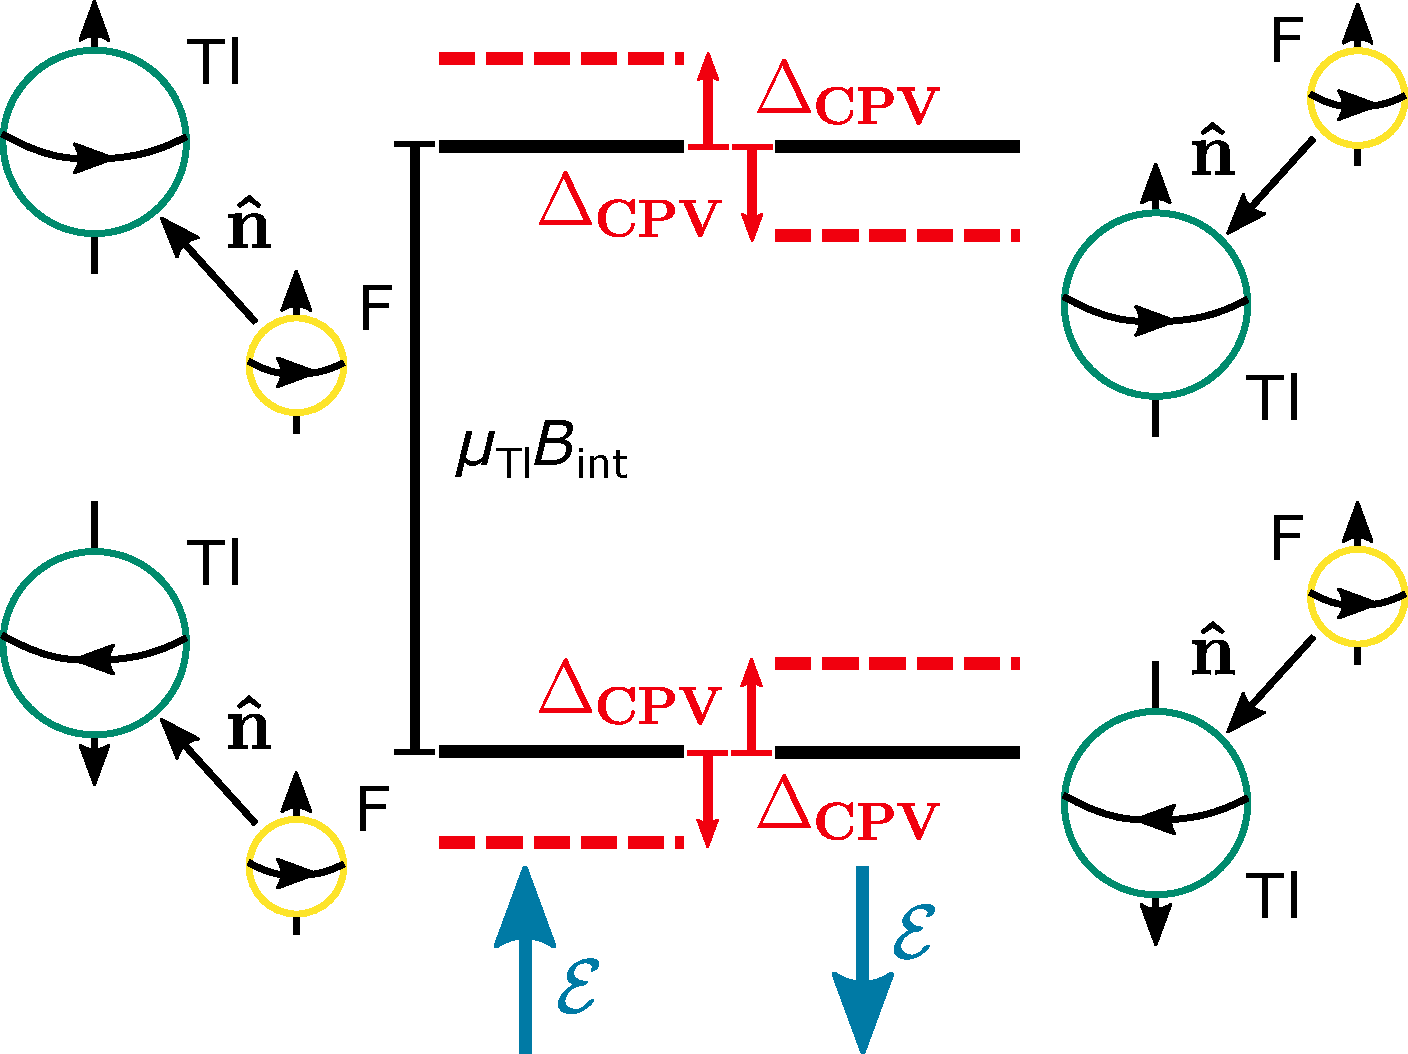
\includegraphics[width=0.48\textwidth,unit=1mm]{figs/svg/edm_levels_pdf_version.pdf}
	\caption{T-violating energy shift $\Delta_{\rm CPV} = W_SS\,\mathcal{P}$ as a result of a nonzero NSM $S$ given by the effective interaction $\mathcal{H}_\text{CPV}= W_S S\vec{I}\cdot \hat{\vec{n}}/I$ (Eq.~\ref{eq:Hamiltonian_effective_interaction}), shown for opposite orientations of the applied field $\Evec$. Here $\mu_1$ is the Tl magnetic moment and $B_1^\mathrm{int}$ is the effective internal magnetic field at the Tl nucleus due to the spin-rotation interaction.
	}
	\label{fig:edm_shift}
\end{figure}

Polar molecules can be polarized readily in laboratory-scale fields owing to their small rotational level separation ($\sim\!10^{-4}\eV$), giving them near-maximal energy shifts induced by a given Schiff moment. Thus, Sandars \cite{sandars1967measurability} suggested a molecular-beam resonance experiment could be used to probe the existence of the proton EDM, if the molecule has a heavy atom with an unpaired proton in the nucleus, such as $^{205}\mathrm{Tl}$. The value of $S$ is determined by measuring energy splittings between spin-up and -down states relative to $\left\langle \hat{\vec{n}}\right\rangle$ (which is parallel to the applied electric field $\bm{\mathcal{E}}$). This splitting will increase or decrease as $\bm{\mathcal{E}}$ (and hence $\left\langle \hat{\vec{n}}\right\rangle$) reverses, due to the interaction in Eq.~\ref{eq:Hamiltonian_effective_interaction}. The difference in level splittings is proportional to the electric polarization $\mathcal{P}$, the interaction strength $W_S$, and $S$ (Fig. \ref{fig:edm_shift}).

\CENTREX\ uses a cold beam of thallium fluoride (TlF) to measure nuclear $T$-violation due to the NSM of the $^{205}$Tl nucleus. It is a suitable system to look for $P$- and $T$-violating interactions for a number of reasons: a molecular beam of thallium fluoride can be readily obtained; many of the molecular states and transitions are known experimentally; the species is a polar diatomic molecule, enhancing the electron density gradient at the site of the nuclei (and hence $W_S$). As the thallium nucleus is heavy $\left(A=205,\,Z=81\right)$ and the NSM-induced energy shift scales $\propto A^{2/3}Z^2$, the observable effect of the Tl Schiff moment is correspondingly large \cite{sandars1967measurability, wilkening1984search}. Since the Tl nucleus contains an unpaired proton,
%the different linear combinations of underlying CPV parameters means
\CENTREX\ will be primarily sensitive to proton EDM effects, as opposed to other leading experiments which are more sensitive to the
%effects associated with neutron spin such as
neutron EDM \cite{graner2016reduced}. TlF is not very sensitive to the electron EDM due to its zero total electron spin \cite{kozlov1995parity}. 

The current best constraint on $T$-violating interactions associated with $S\left(^{205}\mathrm{Tl}\right)$ was found by Cho, Sangster and Hinds in 1991 \cite{cho1989tenfold, cho1991search}, who measured a NSM-induced frequency shift of $\Delta E = 2\Delta_{\rm CPV} = \left(1.4\pm 2.4\right)\times 10^{-4}$~Hz, consistent with zero.\footnote{Throughout, we express both frequencies and energies in linear frequency units (Hz), and all angular momentum operators are treated as dimensionless.} 
Using the effective interaction $\mathcal{H}_\text{CPV}$, the shift in the energy splitting between states with Tl spin up versus spin down, relative to the quantization axis, can be interpreted as
\begin{equation}
    \Delta E= 2 \Delta_{\rm CPV} = 2 W_S\,S\, \textrm{sgn}(\Esca) \,\mathcal{P},
    \label{eq:frequency_shift_due_to_NSM}
\end{equation}
where $W_S = 40539\,$a.u.,
polarization $\mathcal{P} = \langle\hat{\vec{n}} \cdot \hat{\Evec}\rangle = 0.547$, and the sign of $\Esca$ refers to the direction of $\Evec$ relative to a fixed quantizing axis $\hat{z}$.  This determines the Schiff moment \cite{PhysRevA.101.042501, PhysRevLett.88.073001}
\begin{equation}
    S\left(^{205}\mathrm{Tl}\right) = \left(3.6\pm 6.1\right)\times 10^{-11}\,e\,\mathrm{fm}^3.
\end{equation}
With Eq.~\ref{eq:schiff_contributions}, the following limits can be placed:
\begin{equation}
    \label{eq:prev_best_lims}
    \begin{split}
        \bar{\theta} & = \left(1.3 \pm 2.3\right)\ee{-9}, \\
        12\bar{d}_d+9\bar{d}_u & = \left(3.6\pm 6.1\right)\ee{-24}\,\mathrm{cm}, \\
        d_p          & = \left(0.9 \pm 1.5\right)\ee{-23}\,e\,\mathrm{cm},\\
        0.13g\bar{g}_0 - 0.004g\bar{g}_1-0.27g\bar{g}_2 & = \left(3.6 \pm 6.1\right)\ee{-11}.
    \end{split}
\end{equation}
\CENTREX\ aims to improve on these limits by using a cryogenic molecular beam source to achieve a cold beam with higher intensity and lower velocity spread compared to the jet source used in the previous work. Rotational cooling will be performed with optical and microwave pumping, collapsing much of the initial Boltzmann distribution into one state, greatly enhancing the number of molecules accessible for measurement. Finally, optical cycling will be used to assist state readout, resulting in near-unity detection efficiency. Fluorescence detection, compared to the hot-wire techniques used previously, allows for background-free detection if scattered light is well controlled.

\subsection{Thallium Fluoride}
\label{sec:tlf_theory}

\begin{figure}
	    % for axis breaks
    \usetikzlibrary{decorations.markings}
    \def\MarkLt{4pt}
    \def\MarkSep{2pt}
    \tikzset{
      TwoMarks/.style={
        postaction={decorate,
          decoration={
            markings,
            mark=at position #1 with
              {
                  \begin{scope}[xslant=0.2]
                  \draw[line width=\MarkSep,white,-] (0pt,-\MarkLt) -- (0pt,\MarkLt) ;
                  \draw[-] (-0.5*\MarkSep,-\MarkLt) -- (-0.5*\MarkSep,\MarkLt) ;
                  \draw[-] (0.5*\MarkSep,-\MarkLt) -- (0.5*\MarkSep,\MarkLt) ;
                  \end{scope}
              }
           }
        }
      },
      TwoMarks/.default={0.5},
    }

\begin{tikzpicture}[scale=5]

   % length of energy level diagram lines
   \def\len{.05}

   % x-position and length and x-offset of the y-axis labels
   \def\pos{-18}
   \def\lenmark{.025}
   \def\xoffset{.18}

   % x coordinates for m = -2, ... 2
   \def\xa{-4.5*\len}
   \def\xb{-2.5*\len}
   \def\xc{-0.5*\len}
   \def\xd{+1.5*\len}
   \def\xe{+3.5*\len}
   \def\xf{-6.5*\len}
   \def\xg{+5.5*\len}

   % y offset for J = 1, 2
   \def\yA{.6}
   \def\yB{\yA+.7}

   % axis
   \draw[->,TwoMarks=0.2,TwoMarks=0.6] (\xf-\len-\xoffset, -.1)
      -- (\xf-\len-\xoffset,\yB+.25) node[above, xshift = -20] {$E$ [kHz]};

   % brace position
   \def\bracePos{\xg+3*\len}

    
   % J=0 labels
   \draw [decorate,decoration={brace,amplitude=5pt,mirror,raise=4pt},yshift=0pt]
      (\bracePos,-.08) -- node (midJ0) {} (\bracePos,.08) node [black,midway,anchor=west,xshift=25] (nodeJ0) {$0$};
   \draw (\xf-\len-0.5*\lenmark-\xoffset, -.003325) node[anchor=east,below,xshift=\pos]
      {-3.325} -- (\xf-\len+0.5*\lenmark-\xoffset,-.003325) node[right,below,xshift=-\pos] {$1$};
   \draw (\xf-\len-0.5*\lenmark-\xoffset, .009975) node[anchor=east,above,xshift=\pos]
      {9.975} -- (\xf-\len+0.5*\lenmark-\xoffset,.009975) node[right,above,xshift=-\pos] {$0$};

   % J=0 lines
   \draw (\xc, -0.003325) -- (\xc+\len, -0.003325);
   \draw (\xb, -0.003325) -- (\xb+\len, -0.003325);
   \draw (\xd, -0.003325) -- (\xd+\len, -0.003325);
   \draw (\xc, 0.009975) -- (\xc+\len, 0.009975);

   % J=1 labels
   \draw [decorate,decoration={brace,amplitude=10pt,mirror,raise=4pt},yshift=0pt]
      (\bracePos,\yA-.2) -- node (midJ1) {} (\bracePos,\yA+.1) node [black,midway,anchor=west,xshift=25] (nodeJ1) {$1$};
   \draw (\xf-\len-0.5*\lenmark-\xoffset, \yA-.143745) node[anchor=east,below,xshift=\pos] {-143.745} --
      (\xf-\len+0.5*\lenmark-\xoffset,\yA-.143745) node[right,below,xshift=-\pos] {$0$};
   \draw (\xf-\len-0.5*\lenmark-\xoffset, \yA-.121506) node[anchor=east,above,xshift=\pos] {-121.506} --
      (\xf-\len+0.5*\lenmark-\xoffset,\yA-.121506) node[right,above,xshift=-\pos] {$1$};
   \draw (\xf-\len-0.5*\lenmark-\xoffset, \yA+.054446) node[anchor=east,below,xshift=\pos] {54.446} --
      (\xf-\len+0.5*\lenmark-\xoffset,\yA+.054446) node[right,below,xshift=-\pos] {$1$};
   \draw (\xf-\len-0.5*\lenmark-\xoffset, \yA+.068985) node[anchor=east,above,xshift=\pos] {68.985} --
      (\xf-\len+0.5*\lenmark-\xoffset,\yA+.068985) node[right,above,xshift=-\pos] {$2$};

   % J=1 lines
   \draw (\xc, \yA-.143745) -- (\xc+\len, \yA-.143745);
   \draw (\xc, \yA-.121506) -- (\xc+\len, \yA-.121506);
   \draw (\xb, \yA-.121506) -- (\xb+\len, \yA-.121506);
   \draw (\xd, \yA-.121506) -- (\xd+\len, \yA-.121506);
   \draw (\xc, \yA+.054446) -- (\xc+\len, \yA+.054446);
   \draw (\xb, \yA+.054446) -- (\xb+\len, \yA+.054446);
   \draw (\xd, \yA+.054446) -- (\xd+\len, \yA+.054446);
   \draw (\xc, \yA+.068985) -- (\xc+\len, \yA+.068985);
   \draw (\xb, \yA+.068985) -- (\xb+\len, \yA+.068985);
   \draw (\xd, \yA+.068985) -- (\xd+\len, \yA+.068985);
   \draw (\xa, \yA+.068985) -- (\xa+\len, \yA+.068985);
   \draw (\xe, \yA+.068985) -- (\xe+\len, \yA+.068985);

   % J=2 labels
   \draw [decorate,decoration={brace,amplitude=10pt,mirror,raise=4pt},yshift=0pt]
      (\bracePos,\yB-.27) -- node (midJ2) {} (\bracePos,\yB+.18) node [black,midway,anchor=west,xshift=25] (nodeJ2) {$2$};
   \draw (\xf-\len-0.5*\lenmark-\xoffset, \yB-.217455)
   node[anchor=east,left,yshift=-5] {-217.455}
      -- (\xf-\len+0.5*\lenmark-\xoffset,\yB-.217455) node[right,below,xshift=-\pos] {$1$};
   \draw (\xf-\len-0.5*\lenmark-\xoffset, \yB-.172936)
   node[anchor=east,left,yshift=5] {-172.936}
      -- (\xf-\len+0.5*\lenmark-\xoffset,\yB-.172936) node[right,above,xshift=-\pos] {$2$};
   \draw (\xf-\len-0.5*\lenmark-\xoffset, \yB+.105876)
   node[anchor=east,left,yshift=-5] {105.876}
      -- (\xf-\len+0.5*\lenmark-\xoffset,\yB+.105876) node[right,below,xshift=-\pos] {$2$};
   \draw (\xf-\len-0.5*\lenmark-\xoffset, \yB+.141095)
   node[anchor=east,left,yshift=5] {141.095}
      -- (\xf-\len+0.5*\lenmark-\xoffset,\yB+.141095) node[right,above,xshift=-\pos] (J2F3label) {$3$};

   % J=2 lines
   \draw (\xc, \yB-.217455) -- (\xc+\len, \yB-.217455);
   \draw (\xb, \yB-.217455) -- (\xb+\len, \yB-.217455);
   \draw (\xd, \yB-.217455) -- (\xd+\len, \yB-.217455);
   \draw (\xc, \yB-.172936) -- (\xc+\len, \yB-.172936);
   \draw (\xb, \yB-.172936) -- (\xb+\len, \yB-.172936);
   \draw (\xd, \yB-.172936) -- (\xd+\len, \yB-.172936);
   \draw (\xa, \yB-.172936) -- (\xa+\len, \yB-.172936);
   \draw (\xe, \yB-.172936) -- (\xe+\len, \yB-.172936);
   \draw (\xc, \yB+.105876) -- (\xc+\len, \yB+.105876);
   \draw (\xb, \yB+.105876) -- (\xb+\len, \yB+.105876);
   \draw (\xd, \yB+.105876) -- (\xd+\len, \yB+.105876);
   \draw (\xa, \yB+.105876) -- (\xa+\len, \yB+.105876);
   \draw (\xe, \yB+.105876) -- (\xe+\len, \yB+.105876);
   \draw (\xc, \yB+.141095) -- (\xc+\len, \yB+.141095);
   \draw (\xb, \yB+.141095) -- (\xb+\len, \yB+.141095);
   \draw (\xd, \yB+.141095) -- (\xd+\len, \yB+.141095);
   \draw (\xa, \yB+.141095) -- (\xa+\len, \yB+.141095);
   \draw (\xe, \yB+.141095) -- (\xe+\len, \yB+.141095);
   \draw (\xf, \yB+.141095) -- (\xf+\len, \yB+.141095);
   \draw (\xg, \yB+.141095) -- (\xg+\len, \yB+.141095);

   % microwave energies
   \draw[Latex-Latex] (nodeJ0) -- node[above,sloped] {13.3 GHz} (nodeJ1);
   \draw[Latex-Latex] (nodeJ1) -- node[above,sloped] {26.7 GHz} (nodeJ2);

   % approximate F1 labels
   \def\FposX{-5}
   \def\FposY{15}
   \def\FposYY{22}
   \node[xshift=\FposX] at (midJ0) {\nicefrac{1}{2}};
   \node[xshift=\FposX,yshift=-\FposY] at (midJ1) {\nicefrac{1}{2}};
   \node[xshift=\FposX, yshift=\FposY] at (midJ1) {\nicefrac{3}{2}};
   \node[xshift=\FposX,yshift=-\FposYY] at (midJ2) {\nicefrac{3}{2}};
   \node[xshift=\FposX, yshift=\FposYY] at (midJ2) {\nicefrac{5}{2}};
   \node[xshift=\FposX, yshift=47] at (midJ2) (F1label) {$F_1$};
    
   \node at (F1label -| nodeJ2) {$J$};
   \node at (F1label -| J2F3label) {$F$};

\end{tikzpicture}

	\caption{Hyperfine structure in the lowest three rotational levels in the TlF ground state $X^1\Sigma^+$, with no applied fields. Rotational energies $hBJ(J+1)$ should be added to
	%are subtracted from
	the hyperfine energy shifts indicated on the axis. Note the $(2F+1)$-fold degeneracy of each state with total angular momentum $F$, corresponding to the quantum numbers $m_F=-F,\dots,0,\dots,F$.}
	\label{fig:level_diagram}

\end{figure}

The TlF molecule is described by its electronic, vibrational and rotational motion, plus the states of the Tl and F nuclear spins. \CENTREX\ makes use of states both in the vibronic ground state, $X ^1\Sigma^+\left(\nu=0\right)$, and in an electronically excited state, $B ^3\Pi_1\left(\nu=0\right)$.  In both cases, we describe the angular momentum couplings in a Hund's case (a) basis. We typically write energy eigenstates in terms of the basis states $\ket{\eta,J,F_1,F,m_F}$. Here, $\eta$ represents the vibronic quantum numbers; $J$ is the total angular momentum excluding the nuclear spins, $\vec{F}_1 = \vec{J}+\vec{I}_\mathrm{1}$, with $I_\mathrm{1}=1/2$ for $^{205}$Tl; $\vec{F} = \vec{F}_1+\vec{I}_\mathrm{2}$ is the total angular momentum, with $I_\mathrm{2}=1/2$ for $^{19}$F; and $m_F$ is its projection along a quantization axis in the lab frame. Field-free eigenstates are close to these basis states in the ground $X ^1\Sigma^+$ state.  In the $B ^3\Pi_1$ state, strong hyperfine interactions significantly mix states with different $J$ and $F_1$ values. Hence, we describe these eigenstates with the modified notation $\ket{\eta',\widetilde{J}' ,\widetilde{F}_1^\prime,F',m_F'}$, where $\widetilde{J}'$ and $\widetilde{F}_1^\prime$ correspond to the largest component in their basis-state decomposition; the primes indicate that the ket refers to the excited state $B ^3\Pi_1$.

Molecules in the beam are assumed to be in the vibronic ground state, since the beam temperature is much lower than the energy scales associated with the electronic and vibrational excitations. However, even at cryogenic temperatures, there is a Boltzmann distribution over many rotational and nuclear spin states. The dominant term in the energy of rotational/spin levels in the $X ^1\Sigma^+$ state is due to rotation; the mean energy of states with quantum number $J$ is $E_\mathrm{rot}=BJ(J+1)$, where $B\approx 6.67\GHz \approx 0.3\kelvin\,\kB$, where $\kB$ the Boltzmann constant.\footnote{In Ramsey et al.\ \cite{wilkening1984search}, the symbol $B$ denotes the rotational constant in equilibrium position, i.e., there $B\equiv B_\text{e}$. However, the effective $v=0$ rotational constant, $B_0$, is more relevant to \CENTREX. To first order in the Dunham expansion \cite{huber2013molecular}, $B_0=B_\text{e}-\alpha_\text{e}/2$. With $B_\text{e}$ and $\alpha_\text{e}$ from the NIST database \cite{afeefy2011nist}, we find $B_0$. We define the symbol $B\equiv B_0$; its value is shown in Table~\ref{tab:hyperfine_hamiltonian}.}

Hyperfine interactions split sublevels with different $F$ values ($F=J-1,J,J, J+1$, except $F=0,1$ only for $J=0$) in each rotational state. Thus, each rotational level has $4(2J+1)$ magnetic sublevels. %including nuclear spins.
Including rotation, spin-rotation and spin-spin interactions, plus interactions with external electric $(\Evec)$ and magnetic $(\Bvec)$ fields, the system is described by the effective Hamiltonian \cite{wilkening1984search}
\small
$\mathcal{H}_\text{TlF} = \mathcal{H}_\text{rot}+\mathcal{H}_\text{sr}+\mathcal H_\text{ss} + \mathcal H_\text{S}+\mathcal H_\text{Z}$, 
\normalsize
where
\begin{equation} 
    \label{eq:hyperfine_hamiltonian}
    \begin{split}
        \mathcal H_\text{rot} & = B \vec{J}^2 \\
        \mathcal H_\text{sr}&=c_1(\vec I_1\cdot\vec J)+c_2(\vec I_2\cdot\vec J), \\
        \mathcal H_\text{ss}&=c_3 T^2(\vec C)\cdot T^2(\vec I_1, \vec I_2)+c_4(\vec I_1\cdot\vec I_2), \\
        \mathcal H_\text{S}&=-\vec\mu_e\cdot\vec \Evec,\\
        \mathcal H_\text{Z}&=-\frac{\mu_J}{J}(\vec J\cdot\vec \Bvec)-\frac{\mu_1}{I_1}(\vec I_1\cdot\vec \Bvec)-\frac{\mu_2}{I_2}(\vec I_2\cdot\vec \Bvec).
    \end{split}
\end{equation}
Here, the first term in the spin-spin interaction ($\mathcal H_\text{ss}$) contains the scalar product of two rank-2 tensors: one constructed from the modified spherical harmonics $\vec C$, and one from $\vec{I}_1$ and $\vec{I}_2$ \cite{brown2003rotational}. (The matrix elements diagonal in $J$ of this term are given in \cite{wilkening1984search}.)  The hyperfine parameters $c_1,c_2,c_3,c_4$, rotational constant $B$, magnetic moments $\mu_J,\mu_1,\mu_2$, and molecule-frame electric dipole moment $\mu_e$ are all known from previous measurements; their values are given in  Table~\ref{tab:hyperfine_hamiltonian}. A level diagram of low-lying states in the absence of applied fields is shown in Fig.~\ref{fig:level_diagram}.

\begin{table}
    \small
    \setlength\extrarowheight{3pt}
    \rowcolors{2}{white}{gray!25}
	\centering
	\caption{Constants describing rotational, hyperfine, Zeeman, and Stark interactions in the effective TlF ground-state  Hamiltonian (Eq.~\ref{eq:hyperfine_hamiltonian}). All values taken from Ramsey et al.\ \cite{wilkening1984search}, except for $B$ (see Sec. \ref{sec:tlf_theory}).}
	\label{tab:hyperfine_hamiltonian}
	\begin{tabular}{r@{\hspace{5pt}}c@{\hspace{5pt}}l@{\hspace{5pt}}l | r@{\hspace{5pt}}c@{\hspace{5pt}}l@{\hspace{5pt}}l}
    	\toprule
		$B$ & = &           $6.66733$ &     GHz &       $\mu_e$ & = & $4.2282(8)$ &     Debye \\
		$\mu_J$ & = &       $35(15)$ &      Hz/G &      $c_1$ & = & $126.03(12)$ &    kHz \\
		$\mu_1^{205}$ & = & $1.2405(3)$ &   kHz/G &     $c_2$ & = & $17.89(15)$ &     kHz\\
		$\mu_1^{203}$ & = &  $1.2285(3)$ &   kHz/G &     $c_3$ & = & $0.70(3)$ &       kHz \\
		$\mu_2$ & = &      $2.00363(4)$ &  kHz/G  &    $c_4$ & = & $-13.30(72)$ &    kHz \\
		\bottomrule
	\end{tabular}
\end{table}

%%%%%%%%%%%%%%%%%%%%%%%%%%%%%%%%%%%%%%%%%%%%%%55%%%%%%%%%%%%%%%
In \CENTREX, lasers are tuned to $X^1\Sigma^+(\nu=0)\rightarrow B^3\Pi_1\left(\nu=0\right)$ transitions in order to manipulate and read out ground state hyperfine and rotational sublevels. Details of the $B ^3\Pi_1$ state structure are given in \cite{norrgard2017hyperfine,PhysRevA.101.042506}.  Here, only a few main features of the $B$ state substructure are important.  First, the $B$ state hyperfine splittings are very large ($\gtrsim 100\MHz$) compared to the natural linewidth of the transition ($\gamma_B \approx 1.6\MHz$), which is in turn much larger than the ground-state hyperfine splittings ($c_j \lesssim 100\kHz$). This means that hyperfine structure is fully resolved in the excited state, and entirely unresolved in the ground state. Hence, optical transitions in TlF drive a large manifold of ground-state hyperfine levels (with a given value of $J$) to a single hyperfine state with (nominal) quantum numbers $\tilde{J},\tilde{F}_1$ and exact quantum number $F$. Another important feature of the $B$ state is that its matrix of Franck-Condon factors (FCFs) for decay to the $X$ state is extremely diagonal \cite{hunter2012prospects}, such that $\sim\! 99\%$ of the time, the $B(v=0)$ vibronic state decays back to the vibronic ground state $X(v=0)$.  This enables optical pumping and optical cycling with little loss.  However, the mixing of $J$ and $F_1$ by the strong $B$-state hyperfine interaction substantially modifies rotational selection rules in $B-X$ decays, and must be taken into account when describing optical excitation and emission in TlF.

\subsection{TlF in \texorpdfstring{$\Esca$}{E}-fields}
\label{sec:TlF_in_E_fields}

\begin{figure*}
	\centering
	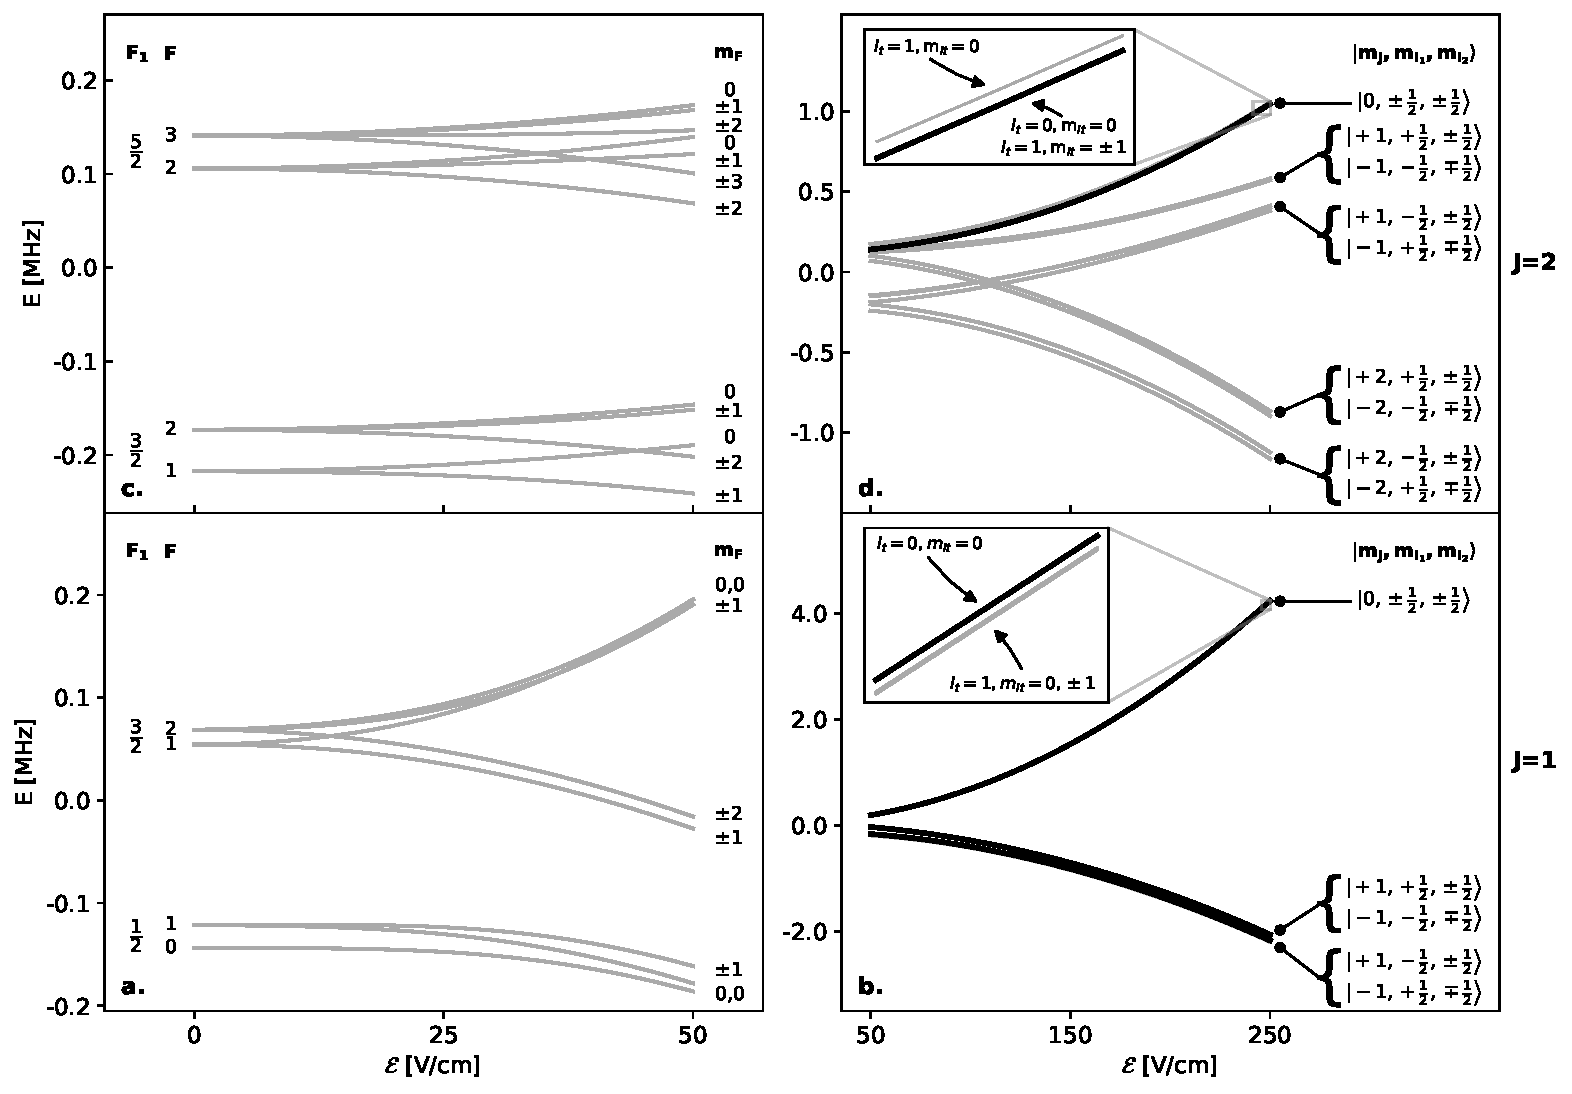
\includegraphics[width=\textwidth]{figs/matplotlib/low_to_mid_field.pdf}
	\caption{Overview of the energy eigenstates for changing $\Esca$-field magnitudes. The low-field regime, where $\Delta E_{\rm S} \ll E_{\rm hf}$, where energy eigenstates retain $J$, $F$, and $F_1$ as approximate quantum numbers is shown in \part{a} for $J=1$ and \part{c} for $J=2$. The mid-field regime, where $E_{\rm hf} \ll \Delta E_{\rm S} \ll E_{\rm rot}$, where both $J$ and $m_J$ are approximate quantum numbers is shown in \part{b} for $J=1$ and \part{d} for $J=2$. States used in \CENTREX\ are shown in bold.}
	\label{fig:low_to_mid_field}
\end{figure*}

\begin{figure}
	\centering
	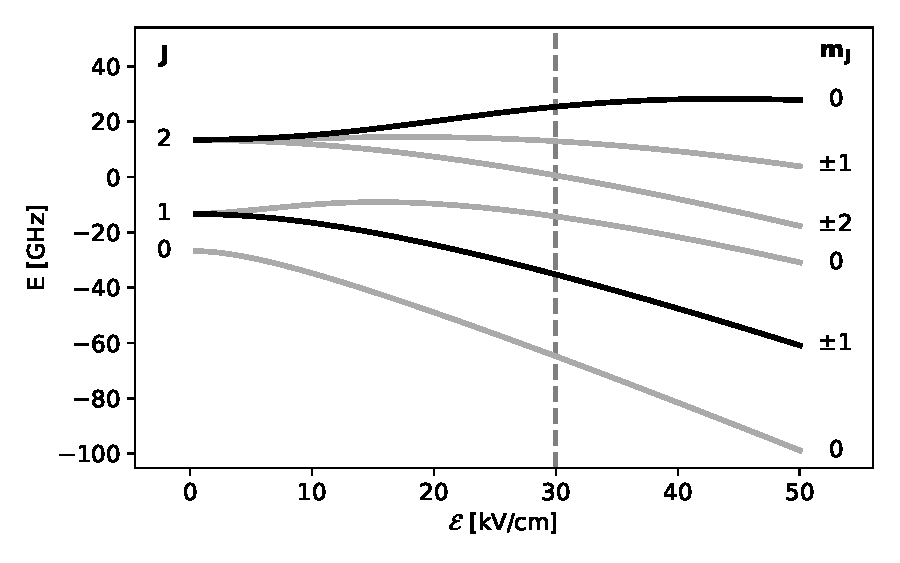
\includegraphics[width=\textwidth/2]{figs/matplotlib/low_to_high_field.pdf}
	\caption{Evolution of the energy eigenstates of the TlF Hamiltonian (Eq. \ref{eq:hyperfine_hamiltonian}) for $\Esca$ ranging from $0\,$V/cm to $50\,$kV/cm, for $J=0,1,2$. States used in \CENTREX\ are shown in bold. Hyperfine structure is unresolved in this plot.}
	\label{fig:low_to_high_field}
\end{figure}

Throughout most of the \CENTREX\ apparatus, TlF molecules experience a non-zero $\Esca$-field and (nominally) zero $\Bsca$-field.
The character of the energy eigenstates changes significantly depending on the $\Esca$-field magnitude, which varies dramatically between stages of the experiment. Hence, it is useful to describe the energy eigenstates of the TlF electronic ground state in different regimes of $\Esca$-field strength (with $\Bsca = 0$), as defined by the ratio of Stark shifts, $\Delta E_{\rm S} = \langle \mathcal{H}_{\rm S}\rangle \sim \mu_e^2 \Esca^2/B$, to the strength of hyperfine interactions, $E_{\rm hf} = \langle \mathcal{H}_{\rm sr} + \mathcal{H}_{\rm ss}\rangle \sim c_j$, or rotational energies, $E_{\rm rot} = \langle \mathcal{H}_{\rm rot}\rangle \sim B$. In all regimes, the total angular momentum projection $m_F$ along 
a space-fixed quantization axis $\hat{z}$ (always defined such that $\Evec$ is very nearly parallel to $\hat{z}$), is an exact quantum number.

In the low-field regime, where $\Delta E_{\rm S} \ll E_{\rm hf}$, energy eigenstates retain $J$, $F$, and $F_1$ as approximate quantum numbers. 
In the mid-field regime, where $E_{\rm hf} \ll \Delta E_{\rm S} \ll E_{\rm rot}$, both $J$ and $m_J$ are approximate quantum numbers. 
Here, the tensor part of the Stark shifts gives rise to energy splittings between levels with different values of $|m_J|$ that are comparable in size to the scalar shifts, i.e., of order $\Delta E_{\rm S}$.  Thus, when $m_J\neq 0$, $\vec{J}$ is strongly coupled to $\Evec$ (and hence to the molecular axis $\vec{\hat{n}}$) by this Stark interaction. In this case, each nuclear spin is coupled to $\vec{J}$ (and thus also to $\Evec$) by the spin-rotation interactions of $\mathcal{H}_{\rm sr}$. Hence, here $m_{I_1}$ and $m_{I_2}$ are approximate quantum numbers. By contrast, in states where $m_J=0$ (including when $J=0$) in this regime, $\left\langle \mathcal{H}_{\rm sr}\right\rangle$ vanishes to first order, and the nuclear spins do not couple to $\vec{J}$ and $\Evec$. However, the nuclear spins remain coupled to each other via the spin-spin interaction $\mathcal{H}_{\rm ss}$.  So, here the total nuclear spin $\vec \It = \vec I_1 + \vec I_2$ and its projection $m_{\It}$ are approximate quantum numbers in addition to $J$ and $m_J=0$. 
Finally, in the high-field regime where $E_{\rm hf} \ll E_{\rm rot} \lesssim \Delta E_{\rm S}$, $J$ states are strongly mixed, and separations between $m_J$ states are on the order of $E_{\rm rot}$. Here, eigenstates are defined by the same approximate quantum numbers as in the mid-field regime, aside from $J$. We refer to these strongly mixed states with the label $\widetilde{J}$, which corresponds to the value of $J$ that any given state connects to adiabatically, if the $\Esca$-field is reduced.
Table \ref{tab:E_field_regimes} summarizes the different regimes and associated eigenstates.  
\begin{table*}[t]
    \centering
    \def\colseplarge{4ex} % should only be used in this table
	\begin{tabular}{@{}r@{\hspace{\colseplarge}}r@{$\,\Delta E_{\rm S}\,$}l@{\hspace{\colseplarge}}r@{$\,\Esca\,$}l@{\hspace{\colseplarge}}>{\raggedright\arraybackslash}m{4cm}@{}}
    	\toprule
    	Regime & \multicolumn{2}{c}{Definition} & \multicolumn{2}{c}{Field strength} & Approx. eigenstates \\
		\midrule
		 Low
		 & & $\ll E_{\rm hf}$
		 & & $\lesssim 50 \Vcm$
		 & $\ket{J,F_1,F,m_F}$ \\\addlinespace[2ex]
		 %
	     Mid
	     & $E_{\rm hf} \ll$ & $\ll E_{\rm rot}$
	     & $50 \Vcm \ll$ & $\lesssim 5 \kVcm$
	     & $\ket{J,m_J \neq 0}\ket{m_{I_1},m_{I_2}}$ 
	       $\ket{J,m_J=0}\ket{\It,m_{\It}}$ \\\addlinespace[2ex]
	     %
	     High
	     & $E_{\rm hf} \ll E_{\rm rot} \lesssim$ &
	     & $5\kVcm \ll$ &
	     & $\ket{\widetilde{J},m_J\neq 0} \ket{m_{I_1},m_{I_2}}$
	       $\ket{\widetilde{J},m_J=0}\ket{\It,m_{\It}}$ \\
		\bottomrule
	\end{tabular}
	\caption{Regimes of electric field strength and associated eigenstates in TlF.}
	\label{tab:E_field_regimes}
\end{table*}


Figure \ref{fig:low_to_mid_field} shows how the relevant energies and eigenstates evolve from the low-field to the mid-field regime for $J=1$ and $J=2$ states.  Bold curves are states directly relevant to \CENTREX. Figure \ref{fig:low_to_high_field} shows a zoom out of states up to $J=2$ from low to high fields.

The $^{205}$Tl NSM measurement is carried out in $\tilde{J} = 1,\, m_J = \pm1$ states of TlF at large electric field $\mathcal{E} = 30$ kV/cm. This choice of states takes advantage of the structure of TlF in electric fields, in two ways. First, the observable energy shift associated with $S$, $\Delta E$, scales linearly with the degree of polarization $\mathcal{P}$ of the TlF molecule (Eq. \ref{eq:frequency_shift_due_to_NSM}). An electric field more easily polarizes states with low $J$, since $\mathcal{P}$ arises from mixing between states with different parity and thus different $J$; these states are closest together when $J$ is small. Additionally, as discussed in Sec. \ref{Sec:InternalComagnetometry}, certain dangerous systematic errors in the NSM measurement are dramatically suppressed in the presence of a strong spin-rotation interaction (later referred to as an effective intra-molecular magnetic field). This requires $m_J \neq 0$. The $\tilde{J} = 1,\, m_J = \pm1$ states hence provide the best combination of sensitivity and systematic error suppression in TlF.\footnote{$|\mathcal{P}|$ is larger in the $J=0,m_J = 0$ states, given the same $\Esca$-field value. Hence, the NSM gives larger energy shifts there. However, in these states where $m_J = 0$, the effective intra-molecular magnetic field vanishes.}
    \section{Basic definitions}
\label{sec:preliminary}
This paper considers binary classification boosting. 
We use the same notations as in~\citep{shalev-shwartz+:jml10}. 
Let $S := ((\bm{x}_i, y_i))_{i=1}^m \in (\xset \times \{\pm 1\})^m$ be 
a sequence of $m$-examples, where $\xset$ is some set. 
Let $\hset \subset [-1, +1]^\xset$ be a set of hypotheses. 
For simplicity, we assume $|\hset| = |\{h_1, h_2, \dots, h_n\}| = n$. 
Note that our scheme can use an infinite set $\hset$. 
It is convenient to regard each $h_j \in \hset$ as 
a canonical basis vector $\bm{e}_j \in \mathbb{R}^n$. 
Let $A = (y_i h_j(\bm x_i))_{i, j} \in [-1, +1]^{m \times n}$ 
be a matrix of size $m \times n$. 
We denote $m$-dimensional capped probability simplex as 
$\psimplex{m}_{\nu} := \{ \bm{d} \in [0, 1/\nu]^m \mid \| \bm{d} \|_1 = 1\}$, 
where $\nu \in [1, m]$. 
We write $\psimplex{m} = \psimplex{m}_{1}$ for shorthand. 
For a set $\cset \subset \mathbb R^n$, 
we denote the convex hull of $\cset$ as 
$
    \convhull (\cset) 
        := \left\{
            \sum_{k} w_k \bm{s}_k
            \mid \sum_k w_k = 1, w_k \geq 0,
            \{\bm{s}_k\}_k \subset \cset
        \right\}
$.

Next, we define some properties for convex functions. 
\begin{def.}[smooth function]
    A function $f : \mathbb R^m \to \mathbb R$ is 
    said to be $\eta$-smooth 
    over a convex set $\cset \subset \mathbb R^m$ 
    w.r.t. a norm $\| \cdot \|$ if 
    \begin{align}
        \label{eq:smoothness}
        \forall \bm{x}, \bm{y} \in \cset, \quad
        f(\bm{y}) 
        \leq f(\bm{x}) + (\bm{y} - \bm{x})^\top \nabla f(\bm{x})
        + \frac{\eta}{2} \|\bm{y} - \bm{x}\|^2.
    \end{align}
\end{def.}

Similarly, we define the strongly convex function. 
\begin{def.}[strongly convex function]
    A function $f : \mathbb R^m \to \mathbb R$ is 
    said to be $\eta$-strongly convex 
    over a convex set $C \subset \mathbb R^m$ 
    w.r.t. a norm $\| \cdot \|$ if 
    \begin{align}
        \nonumber
        \forall \bm{x}, \bm{y} \in \cset, \quad
        f(\bm{y}) 
        \geq f(\bm{x}) + (\bm{y} - \bm{x})^\top \nabla f(\bm{x})
        + \frac{\eta}{2} \|\bm{y} - \bm{x}\|^2.
    \end{align}
\end{def.}

We also define Fenchel conjugate. 
\begin{def.}[Fenchel conjugate]
    The Fenchel conjugate $f^\star$ of 
    a function $f : \mathbb{R}^m \to [-\infty, +\infty]$ is defined as
    \begin{align*}
        f^\star(\bm{\theta}) = \sup_{\bm{d} \in \mathbb{R}^m} 
        \left( \bm{d}^\top \bm{\theta} - f(\bm{d}) \right).
    \end{align*}
\end{def.}
It is well known that if $f$ is a $1/\eta$-strongly convex function 
w.r.t. the norm $\|\cdot\|$ for some $\eta > 0$, 
$f^\star$ is an $\eta$-smooth function
w.r.t. the dual norm $\|\cdot\|_\star$. 
Further, if $f$ is a strongly convex function, 
the gradient vector of $f^\star$ is written as
\begin{align}
    \nonumber
    \nabla f^\star(\bm{\theta}) = 
    \arg \sup_{\bm{d} \in \mathbb{R}^m}
    \left( \bm{d}^\top \bm{\theta} - f(\bm{d}) \right).
\end{align}
One can find the proof of these properties 
here~\citep{borwein+:springer06,shalev-shwartz+:jml10}.

\begin{lem.}
    \label{lem:fenchel_conjugate_functions}
    Let $f, \tilde{f} : \mathbb{R}^m \to (-\infty, +\infty]$ be 
    functions such that 
    \begin{align*}
        \exists c > 0, \forall \bm{\theta},
        f(\bm{\theta}) \leq \tilde{f}(\bm{\theta}) \leq f(\bm{\theta}) + c.
    \end{align*}
    Then, 
    $
        f^\star(\bm{\mu}) - c
        \leq \tilde{f}^\star(\bm{\mu})
        \leq f^\star(\bm{\mu})
    $ holds for all $\bm{\mu}$.
\end{lem.}
Finally, we show the duality theorem~\citep{borwein+:springer06}.
\begin{thm.}[\cite{borwein+:springer06}]
    \label{thm:strong_duality}
    Let $f : \mathbb{R}^m \to (-\infty, +\infty]$ and 
    $g : \mathbb{R}^n \to (-\infty, +\infty]$ be convex functions, 
    and a linear map $A : \mathbb{R}^m \to \mathbb{R}^n$. 
    Define the Fenchel problems
    \begin{align}
        \label{eq:strong_duality_primal}
        \gamma & = \inf_{\bm{d}} f(\bm{d}) + g(A^\top\bm{d}), \\
        \label{eq:strong_duality_dual}
        \rho   & = \sup_{\bm{w}} -f^\star(-A \bm{w}) - g^\star(\bm{w}).
    \end{align}
    Then, $\gamma \geq \rho$ holds. 
    Further, $\gamma = \rho$ holds if~\footnote{%
        For a set $\cset \subset \mathbb{R}^n$, %
        $
            \interior(C) = \{
                \bm{w} \in C \mid
                    \forall \bm{v} \in \mathbb{R}^n,
                    \exists t > 0,
                    \forall \tau \in [0, t], \bm{w} + \tau \bm{v} \in C
            \}
        $ and \\ %
        $
            \domain g - A^\top \domain f
            = \{ \bm{w} - A^\top \bm{d} \mid
                \bm{w} \in \domain g,
                \bm{d} \in \domain f
            \}
        $. %
    }
    $\bm{0} \in \interior \left(\domain g - A^\top \domain f\right)$. 
    Furthermore, points $\bar{\bm{d}} \in \psimplex{m}_{\nu}$ and 
    $\bar{\bm{w}} \in \psimplex{n}$ are optimal solutions 
    for problems~(\ref{eq:strong_duality_primal}) 
    and~(\ref{eq:strong_duality_dual}), respectively, 
    if and only if $-A \bar{\bm{w}} \in \partial f(\bar{\bm{d}})$ 
    and $\bar{\bm{w}} \in \partial g(A^\top \bar{\bm{d}})$.
\end{thm.}


With these notations, 
we define the soft margin optimization problem 
as the dual problem of the edge minimization problem. 
The edge minimization problem is defined as 
\begin{align}
    \label{eq:edge_minimization}
    \min_{\bm{d}}
        \max_{j \in [n]} (\bm{d}^\top A)_j
        + f(\bm{d}),
    \quad
    \text{where}
    \quad
    f(\bm{d}) = 
    \begin{cases}
        0 & \bm{d} \in \psimplex{m}_{\nu} \\
        +\infty & \bm{d} \notin \psimplex{m}_{\nu}
    \end{cases}.
\end{align}
The quantity $(\bm{d}^\top A)_j = \sum_{i=1}^m d_i y_i h_j(\bm{x}_i)$ is 
often called the \emph{edge} of the hypothesis $h_j$ 
w.r.t. the distribution $\bm{d} \in \psimplex{m}_{\nu}$. 
\cite{shalev-shwartz+:jml10} showed that 
the $\ell_1$-norm regularized soft margin optimization problem is 
formulated via Fenchel duality as 
\begin{align}
    \label{eq:soft_margin_maximization}
    \max_{\bm w \in \psimplex{n}} - f^\star(- A\bm w)
    = \max_{\bm w \in \psimplex{n}} \min_{\bm{d} \in \psimplex{m}_{\nu}}
    \bm{d}^\top A \bm{w}.
\end{align}
Furthermore, the duality gap between~(\ref{eq:edge_minimization}) 
and~(\ref{eq:soft_margin_maximization}) is zero. 
The soft margin optimization aims 
to find an optimal combined hypothesis 
$H_{T} = \sum_{j=1}^n \bar{w}_j h_j$, 
where $\bar{\bm{w}} \in \psimplex{n}$ is 
an optimal solution of~(\ref{eq:soft_margin_maximization}). 
Although the edge minimization and soft margin optimization problems are 
formulated as a linear program, 
solving the problem for a huge class $\hset$ is hard. 
Boosting is a standard approach to dealing with the problem. 


\subsection{Boosting}
Boosting is a protocol between two algorithms; 
the booster and the weak learner. 
For each iteration $t = 0, 1, 2, \dots, T$, 
the booster chooses a distribution $\bm{d}_t \in \psimplex{m}_{\nu}$ 
over the training examples $S$. 
Then, the weak learner returns a hypothesis $h_{j_{t+1}} \in \hset$ 
to the booster that satisfies $({\bm{d}_t}^\top A)_{j_{t+1}} \geq g$ 
for some unknown guarantee $g > 0$. 
The boosting algorithm aims to produce a convex combination 
$H_T = \sum_{t=1}^T w_{T,j_t} h_{j_t}$ 
of the hypotheses $\{h_{j_1}, h_{j_2}, \dots, h_{j_T}\} \subset \hset$ 
that satisfies 
\begin{align}
    \label{eq:boosting_goal}
    -f^\star ( - A \bm{w}_T )
    = \min_{\bm{d} \in \psimplex{m}_{\nu}} 
    \bm{d}^\top A \bm{w}_T
    = \min_{\bm{d} \in \psimplex{m}_{\nu}} 
    \sum_{i=1}^m d_i y_i H_T(\bm{x}_i)
    \geq g - \epsilon
\end{align}
for any predefined $\epsilon > 0$. 
Suppose that the weak learner always returns a max-edge hypothesis 
for any given distribution $\bm{d} \in \psimplex{m}_{\nu}$. 
In that case, 
the goal is to find an $\epsilon$-approximate solution 
of~(\ref{eq:soft_margin_maximization}). 

\subsection{The Frank-Wolfe algorithms}
We briefly introduce the standard Frank-Wolfe algorithm. 
The original Frank-Wolfe (FW) algorithm is 
a first-order iterative algorithm 
invented by~\cite{marguerite+:nrl56}. 
The FW algorithm solves the problems of the form:
$\min_{\bm{x} \in \cset} f(\bm{x})$, 
where $\cset \subset \mathbb R^m$ is a closed convex set 
and $f : \cset \to \mathbb R$ is an $\eta$-smooth and convex function. 

In each iteration $t$, 
the FW algorithm seeks an extreme point 
$
    \bm{s}_{t+1}
    \in \arg \min_{\bm{s} \in \cset} \bm{s}^\top \nabla f(\bm{x}_t)
$. 
Then, it updates the iterate as 
$\bm{x}_{t+1} = \bm{x}_t + \lambda_t (\bm{s}_{t+1} - \bm{x}_t)$ 
for some $\lambda_t \in [0, 1]$. 
Although the classical result~\citep{marguerite+:nrl56,jaggi:icml13}
suggests $\lambda_t = 2/(t+2)$, 
$\lambda_t$ has many choices. 
% there are many choices of $\lambda_t$. 
For example, one can choose $\lambda_t$ as
\begin{align}
    \label{eq:short_step_update}
    \lambda_t := 
        \clip
        \frac{(\bm{x}_t - \bm{s}_{t+1})^\top \nabla f(\bm{x}_t)}
             {\eta \|\bm{s}_{t+1} - \bm{x}_t\|^2},
\end{align}
where $\clip x = \max\{0, \min\{1, x\}\}$. 
This optimal solution minimizes 
the right-hand side of the inequality~(\ref{eq:smoothness}) 
and is often called the \emph{short-step} strategy.
Alternatively, one can choose 
$
    \lambda_t \in 
    \arg\min_{\lambda \in [0, 1]} 
    f(\bm{x}_t + \lambda (\bm{s}_{t+1} - \bm{x}_t))
$ by line search. 
This step size improve the objective more than the short-step strategy. 
Since the FW algorithm aims to find an optimal solution, 
one can choose $\bm{x}_{t+1}$ by solving the problem:
$
    \bm{x}_{t+1} \gets
    \arg \min_{
        \bm{x} \in \mathop{\rm CH}(\{\bm{s}_1, \dots, \bm{s}_{t+1}\})
    } f(\bm x)
$. 
This update rule is 
called the \emph{Fully Corrective} FW algorithm~(e.g., \cite{jaggi:icml13}). 
Although the fully corrective update yields $\bm{x}_{t+1}$ 
that most decreases the objective over the convex hull, 
it loses the fast computational advantage per iteration.

The FW algorithms converge to 
an $\epsilon$-approximate solution in $O(\eta/\epsilon)$ iterations 
if the objective function is $\eta$-smooth w.r.t. 
some norm over $\cset$~\citep{jaggi:icml13,marguerite+:nrl56}. 
The best advantage of the FW algorithm is the projection-free property; 
there is no projection onto $\cset$, 
so the running time per iteration is 
faster than the projected gradient methods. 


    \paragraph{Sampling CF data.} Sampling in CF-data has been a popular choice for three major scenarios. Most prominently, sampling is used for mining hard-negatives while training recommendation algorithms. Some popular approaches include random sampling; using the graph-structure % to find the hardest negatives 
\cite{pinsage, eclare}; and ad-hoc techniques like similarity search \cite{slice}, stratified sampling \cite{sampling_cf_nn}, \etc % On the other hand, 
Sampling is also generally employed for evaluating recommendation algorithms by estimating expensive to compute metrics like Recall, nDCG, \etc \cite{sampled_metrics, castells_sampling}. Finally, sampling is also used to create smaller sub-samples of 
% the \emph{entire} data 
a big dataset
for reasons like fast experimentation, benchmarking different algorithms, privacy concerns, \etc However, the consequences of different samplers on any of these downstream applications is under-studied, and is the main research interest of this paper. 

\paragraph{Coreset selection.} Closest to our work, a coreset is loosely defined as a subset of data-points that maintains a similar ``quality'' as the full dataset for subsequent model training. Submodular approaches try to optimize a function $f : \mathbf{V} \mapsto \mathcal{R}_+$ which measures the utility of a subset $\mathbf{V} \subseteq \mathbf{X}$, and use it as a proxy to select the best coreset \cite{coreset_1}. More recent works treat coreset selection as a bi-level optimization problem \cite{coreset_bilevel, coreset_bilevel_2} and directly optimize for the best coreset for a given downstream task. Selection-via-proxy \cite{svp} is another technique which employs a base-model as a proxy to tag the importance of each data-point. Note, however, that 
% all of the discussed 
most existing
coreset selection approaches were designed primarily for classification data, whereas adapting them for CF-data is non-trivial because of: (1) the inherent data heterogeneity; the (2) wide range of recommendation metrics; and (3) the prevalent missing-data characteristics.

\paragraph{Evaluating sample quality.} The quality of a dataset sample, if estimated correctly is of high interest for various applications. Short of being able to evaluate the ``true'' utility of a sample, one generally resorts to either retaining task-dependent characteristics \cite{evaluate_sample_quality_1} \emph{or} employing universal, handcrafted features like a social network's hop distribution, eigenvalue distribution, \etc \cite{large_graphs} as meaningful proxies. Note that evaluating the sample quality with a limited set of handcrafted features might introduce bias in the sampled data, depending on the number and quality of such features.

    \section{Main results}
\label{sec:main_result}
We first show 
a unified view of the boosting algorithms 
via Fenchel duality. 
From this view, LPBoost, ERLPBoost, and C-ERLPBoost can be seen as 
instances of the Frank-Wolfe algorithm 
with different step sizes and objectives. 
Using this knowledge, we derive a new boosting scheme. 
\subsection{A unified view of boosting for the soft margin optimization}
This section assumes that the weak learner 
always returns a hypothesis $h \in \hset$ 
that maximizes the edge w.r.t. the given distribution. 
We start by revisiting C-ERLPBoost. 
Recall that C-ERLPBoost (and ERLPBoost) aim to solve the convex program 
\begin{align}
    \label{eq:smoothed_problem}
    \min_{\bm{d}}
    \max_{j \in [n]} (\bm{d}^\top A)_j + \tilde{f}^\star (\bm{d}),
\end{align}
where $\tilde{f} = f + \frac{1}{\eta} \Delta$. 
Since $\frac{1}{\eta} \Delta$ is 
a $\frac{1}{\eta}$-strongly convex function w.r.t. $\ell_1$-norm, 
so does $\tilde{f}$. 
By Fenchel duality, the dual problem is 
\begin{align}
    \label{eq:smoothed_softmargin}
    \max_{\bm{w} \in \psimplex{n}} - \tilde{f}^\star( -A \bm{w} )
    = - \min_{\bm{w} \in \psimplex{n}}
        \tilde{f}^\star( -A \bm{w} )
    = - \min_{\bm{\theta} \in -A\psimplex{n}}
        \tilde{f}^\star(\bm{\theta}),
\end{align}
where $-A \psimplex{n} = \{ -A \bm{d} \mid \bm{d} \in \psimplex{n}\}$, 
with zero duality gap. 
Further, $\tilde{f}^\star$ is an $\eta$-smooth function 
w.r.t. $\ell_\infty$-norm. 
Thus, the soft margin optimization problem becomes 
a minimization problem of a smooth function. 

In each iteration $t$, 
C-ERLPBoost updates the distribution $\bm{d}_t \in \psimplex{m}_{\nu}$ 
over examples as the optimal solution of~(\ref{eq:cerlpb_update}). 
This computation corresponds to the gradient computation 
$\nabla \tilde{f}^\star( \theta_t )$, where $\theta_t = - A\bm{w}_t$. 
Then, obtain a basis vector $\bm{e}_{j_{t+1}} \in \psimplex{n}$ 
corresponding to hypothesis $h_{j_{t+1}} \in \hset$ 
that maximizes the edge; 
$j_{t+1} \in \arg \max_{j \in [n]} (\bm{d}_t^\top A)_j$. 
We can write this calculation regarding the gradient of $\tilde{f}^\star$;
\begin{align*}
    \arg \max_{\bm{e}_j : j \in [n]} \bm{d}_t^\top A \bm{e}_j
    = \arg \min_{\bm{e}_j : j \in [n]}
        (-A\bm{e}_j)^\top \nabla \tilde{f}^\star (\bm{\theta}_t)
    = \arg \min_{\bm{\theta} \in -A\psimplex{n}}
        \bm{\theta}^\top \nabla \tilde{f}^\star (\bm{\theta}_t).
\end{align*}
Thus, finding a hypothesis that maximizes edge corresponds to 
solving linear programming in the Frank-Wolfe algorithm. 
Further, C-ERLPBoost updates the weights as 
$\bm{w}_{t+1} = \bm{w}_t + \lambda_t (\bm{e}_{j_{t+1}} - \bm{w}_t)$, 
where $\lambda_t$ is the short-step~\footnote{%
    They also suggests the line search update. %
    This case yields a better progress than short-step, %
    so the same iteration bound holds. %
}, as in eq.~(\ref{eq:short_step_update}).
From these observations, we can say that the C-ERLPBoost is 
an instance of the Frank-Wolfe algorithm. 
Since $\tilde{f}^\star$ is $\eta$-smooth, we can say that 
this algorithm converges in $O(\eta/\epsilon)$ iterations 
for a max-edge weak learner. 

Similarly, we can say that LPBoost and ERLPBoost are 
instances of the Frank-Wolfe algorithm. 
Let $J_t := \{j_1, j_2, \dots, j_{t} \}$ be the set of indices 
corresponding to the hypotheses $\{h_{j_1}, h_{j_2}, \dots, h_{j_{t}}\}$ 
and $\eset_t := \{ \bm{e}_{j} \mid j \in J_t \}$ be 
the corresponding basis vectors. 
LPBoost and ERLPBoost update the distribution as 
the optimal solutions 
$\bm{d}_t^{\rm{L}} \in \partial f^\star( -A \bm{w}_t^{\rm L})$ 
and $\bm{d}_t^{\rm{E}} = \nabla \tilde{f}^\star (-A \bm{w}_t^{\rm E})$, 
where 
\begin{alignat}{2}
    \label{eq:lpb_weight}
    \text{(LPBoost)} & \quad &
        \bm{w}_t^{\rm{L}} \gets \arg \max_{\bm{w} \in \convhull(\eset_t)}
        - f^\star (-A \bm{w}), \\
    \label{eq:erlpb_weight}
    \text{(ERLPBoost)} & \quad &
        \bm{w}_t^{\rm{E}} \gets \arg \max_{\bm{w} \in \convhull(\eset_t)}
        - \tilde{f}^\star (-A \bm{w}).
\end{alignat}
Therefore, we can say that LPBoost and ERLPBoost are 
instances of the fully-corrective FW algorithm 
for objectives $f^\star$ and $\tilde{f}^\star$, respectively. 
Under the max-edge weak learner assumption, 
one can derive the same iteration bound for ERLPBoost 
since $\tilde{f}^\star$ is $\eta$-smooth. 
We summarize these connections to the following theorem. 
\begin{thm.}
    LPBoost, ERLPBoost, and C-ERLPBoost are instances of the FW algorithm. 
\end{thm.}
%
%
%
%
%
%
%
%
%
%
%
%
\subsection{Generic schemes for margin-maximizing boosting}
\begin{algorithm}[t]
    % \SetAlgoLined
    \caption{A theoretically guaranteed boosting scheme}
    \begin{algorithmic}[1]
        \REQUIRE{%
            Training examples 
            $
                S = \left( (\bm{x}_i, y_i) \right)_{i=1}^m
                \in (\xset \times \{\pm 1\})^m
            $, %
            a hypothesis set $\hset \subset [-1, +1]^\xset$, 
            a FW algorithm $\fwalg$, 
            a secondary algorithm $\secalg$, %
            and parameters $\nu > 0$ and $\epsilon > 0$. %
        }
        \STATE{Set $A = \left(y_i h_j(\bm{x}_i)\right)_{i, j} \in [-1, +1]^{m \times n}$.}
        \STATE{%
            Send $\bm{d}_0 = \frac{1}{m} \bm{1}$ to the weak learner %
            and obtain a hypothesis $h_{j_1} \in \hset$. %
        }

        \STATE{Set $\bm{w}_{1} = \bm{e}_{j_1}$.}

        \FOR{$t=1, 2, \dots, T$}
            \STATE{
                Compute the distribution 
                $
                    \bm{d}_t 
                    = \nabla \tilde{f}^\star(- A \bm{w}_t)
                    = \arg \min_{\bm{d} \in \psimplex{m}_{\nu}}
                    \left[
                    \bm{d}^\top A \bm{w}_t + \frac 1 \eta \Delta (\bm{d})
                    \right]
                $.
            }

            \STATE{%
                Obtain a hypothesis $h_{j_{t+1}} \in \hset$ 
                and the corresponding basis vector 
                $\bm{e}_{j_{t+1}} \in \psimplex{n}$. 
            }

            \STATE{
                Set $
                    \epsilon_t := \min_{0 \leq \tau \leq t}
                    (\bm{d}_\tau^\top A)_{j_{\tau + 1}}
                    + \tilde{f}^\star(- A\bm{w}_t)
                $ and let
                $\eset_{t+1} := \{ \bm{e}_{j_\tau} \}_{\tau=1}^{t+1}$.
            }

            \IF{$\epsilon_t \leq \epsilon / 2$}
                \STATE{Set $T = t$, \textbf{break}.}
            \ENDIF

            \STATE{
                Compute the FW weight 
                $
                    \bm{w}_{t+1}^{(1)}
                    = \fwalg
                    % \left(
                    (
                        A, \bm{w}_{t}, \bm{e}_{j_{t+1}},
                        \eset_{t}, \bm{d}_t
                        % \eset_{t}, \nabla \tilde{f}^\star (-A\bm{w}_t)
                    )
                    % \right)
                $.
            }
            \STATE{%
                Compute the secondary weight %
                $\bm{w}_{t+1}^{(2)} = \secalg(A, \eset_{t+1})$.
            }

            \STATE{
                Update the weight 
                $
                    \bm{w}_{t+1} 
                    \gets \arg \min_{\bm{w}_{t+1}^{(k)}: k \in \{1, 2\}} 
                    \tilde{f}^\star (-A\bm{w}_{t+1}^{(k)})
                $.
            }
        \ENDFOR
        \ENSURE{Combined classifier $H_T = \sum_{t=1}^T w_{T, t} h_t$.}
    \end{algorithmic}
    \label{alg:our_scheme}
\end{algorithm}

\begin{algorithm}[th]
    \begin{algorithmic}[1]
        \REQUIRE{%
            A matrix %
            $
                A = \left( y_i h_j (\bm{x}_i) \right)_{i, j}
                \in [-1, +1]^{m \times n}
            $ %
            and a set of basis vectors $\eset_{t+1} \subset \psimplex{n}$. %
        }

        \ENSURE{%
            $
                \bm{w} \gets \arg\max_{\bm{w} \in \convhull (\eset_{t+1})} 
                    \min_{\bm d \in \psimplex{m}_{\nu}}
                    \bm{d}^\top A \bm{w}
            $.
        }
    \end{algorithmic}
    \caption{LPBoost rule $\secalg (A, \eset_{t+1})$}
    \label{alg:lpb_subroutine}
\end{algorithm}
%
% Short step scheme
%
\begin{algorithm}[th]
    \begin{algorithmic}[1]
        \ENSURE{
            $
                \bm{w}_{t+1}^{(1)} 
                = \bm{w}_t + \lambda_t (\bm{e}_{j_{t+1}} - \bm{w}_t)
            $, where 
            $
                \lambda_t = 
                \clip
                \frac
                    {\bm{d}_t^\top A (\bm{e}_{j+1} - \bm{w}_t)}
                    % {\nabla \tilde{f}^\star(-A\bm{w}_t)^{\top} A (\bm{e}_{j+1} - \bm{w}_t)}
                    {\eta \| A (\bm{e}_{j+1} - \bm{w}_t) \|_{\infty}^2}
            $.
        }
    \end{algorithmic}
    \caption{Short step rule
        $
            \fwalg
            (
                A, \bm{w}_t, \bm{e}_{j_{t+1}},
                \eset_{t}, \bm{d}_t
                % \eset_{t}, \nabla \tilde{f}^\star (-A \bm{w}_t)
            )
        $
    }
    \label{alg:ss_rule}
\end{algorithm}
We propose FW-like boosting schemes 
from the above observations, 
shown in Algorithm~\ref{alg:our_scheme}. 
Algorithm~\ref{alg:our_scheme} takes two update rules, 
a FW update rule $\fwalg$ and 
a secondary update rule $\secalg$. 
Both algorithms return a weight $\bm{w} \in \psimplex{n}$. 
Intuitively, the FW update rule $\bm{w}_t^{(1)}$ is 
a safety net for the convergence guarantee. 
Further, the convergence analysis only depends on 
the FW update $\bm{w}_{t+1}^{(1)}$, 
so that one can incorporate any update rule to $\secalg$. 
For example, one can use the update rule~(\ref{eq:erlpb_weight}) 
as $\secalg(A, \eset_{t+1})$. 
Algorithm~\ref{alg:our_scheme} becomes 
ERLPBoost in this case 
since $\bm{w}_{t+1} = \bm{w}_{t+1}^{(2)}$ holds for any $t$. 
Even though this setting, the convergence guarantee holds 
so that we can prove the same convergence rate for ERLPBoost 
by our general analysis. 

Recall that our primary objective is to find a weight vector $\bm{w}$ 
that optimizes the linear program~(\ref{eq:soft_margin_maximization}). 
The most practical algorithm, LPBoost, 
solves the optimization problem over past hypotheses, 
so using the solution as $\secalg$ is a natural choice. 
Algorithm~\ref{alg:lpb_subroutine} summarizes this update. 
Note that the LPBoost update 
differs from the fully-corrective FW algorithm 
since the objective function is $\tilde{f}^\star$, not $f^\star$. 

Furthermore, as described in~\citep{shalev-shwartz+:jml10}, 
one can compute the distribution 
$\bm{d}_t = \nabla \tilde{f}^\star (-A \bm{w}_t)$ 
by a sorting-based algorithm, 
which takes $O(m \ln m)$ iterations\footnote{%
They also suggest a linear time algorithm, %
see~\citep{herbster+:jmlr01}. %
}. 
Thus, the time complexity per iteration depends on 
the secondary algorithm $\secalg$. 


Before getting into the convergence analysis, 
we first justify the stopping criterion 
in Algorithm~\ref{alg:lpb_subroutine}. 
This criterion is similar to the one in C-ERLPBoost 
but better than it. 
Therefore, our algorithms tend to converge in early iterations. 
\begin{lem.}
    \label{lem:stopping_criterion}
    Let 
    $
        \epsilon_t 
        := \min_{0 \leq \tau \leq t} (\bm{d}_{\tau}^\top A)_{j_{\tau + 1}}
        + \tilde{f}^\star( -A \bm{w}_t)
    $ be the optimality gap defined in Algorithm~\ref{alg:lpb_subroutine} 
    and let $\eta = 2 \ln(m / \nu) / \epsilon$. 
    Then, $\epsilon_t \leq \epsilon / 2$ implies 
    $- f^\star (- A \bm{w}_t ) \geq g - \epsilon$. 
\end{lem.}
\begin{proof}
    By the weak-learnability assumption, 
    $\epsilon_t \geq g + \tilde{f}^\star ( -A \bm{w}_t )$. 
    The statement follows from Lemma~\ref{lem:fenchel_conjugate_functions}.
\end{proof}
Now, we prove the convergence rate for our scheme. 
This theorem shows the same convergence guarantee for 
ERLPBoost and C-ERLPBoost. 
\begin{thm.}[A convergence rate for Algorithm~\ref{alg:our_scheme}]
    \label{thm:mlpboost_convergence_guarantee}
    Assume that the weak learner returns 
    a hypothesis $h_{j_{t+1}} \in \hset$ that satisfies
    $(\bm{d}_t^\top A)_{j_{t+1}} \geq g$ 
    for some unknown guarantee $g$. 
    Let $\fwalg$ be a FW update with 
    classic step $\lambda_t = \frac{2}{t+2}$, or
    short-step as in Algorithm~\ref{alg:ss_rule}. 
    Then, for any secondary algorithm $\secalg$, 
    Algorithm~\ref{alg:our_scheme} converges to 
    an $\epsilon$-accurate solution of~(\ref{eq:soft_margin_maximization}) 
    in $O\left( \frac{1}{\epsilon^2} \ln \frac{m}{\nu} \right)$ iterations. 
\end{thm.}
\begin{proof}
    First of all, we prove the bound for the classic step size. 
    We start by showing the recursion 
    \begin{align}
        \label{eq:convergence_proof_0}
        \epsilon_{t+1}
        \leq (1 - \lambda_t) \epsilon_t + 2 \eta \lambda_t^2.
    \end{align}
    By using the definition of $\bm{w}_{t+1}$ 
    and the $\eta$-smoothness of $\tilde{f}^\star$, 
    \begin{align}
        \epsilon_t - \epsilon_{t+1}
            & \geq \tilde{f}^\star ( -A \bm{w}_t )
                - \tilde{f}^\star ( -A \bm{w}_t^{(1)} ) \nonumber \\
            & = \tilde{f}^\star ( -A \bm{w}_t )
                - \tilde{f}^\star (
                    -A \bm{w}_t + \lambda_t A(\bm{w}_t - \bm{e}_{{j_t+1}})
                ) \nonumber \\
            \label{eq:convergence_proof_1}
            & \geq \lambda_t ( A (\bm{e}_{j_{t+1}} - \bm{w}_{t}) )^\top
                \nabla \tilde{f}^\star (- A \bm{w}_t) - 2\eta \lambda_t^2,
    \end{align}
    where eq.~(\ref{eq:convergence_proof_1}) holds since 
    $A \in [-1, +1]^{m \times n}$ 
    and $\bm{e}_{j_{t+1}}, \bm{w}_t \in \psimplex{n}$. 
    By the non-negativity of the entropy function 
    and the definition of $\bm{d}_t$, we get
    \begin{align}
            \lambda_t ( A (\bm{e}_{j_{t+1}} - \bm{w}_{t}) )^\top
                \nabla \tilde{f}^\star (- A \bm{w}_t)
            & = \lambda_t \bm{d}_t^\top A (\bm{e}_{j_{t+1}} - \bm{w}_{t})
                \nonumber \\
            & \geq \lambda_t
                \left[
                    \min_{0 \leq \tau \leq t} 
                    (\bm{d}_\tau^\top A)_{j_{\tau + 1}} 
                    - \bm{d}_{t}^\top A \bm{w}_t 
                    - \frac{1}{\eta} \Delta (\bm{d}_t)
                \right]
                \nonumber \\
            \label{eq:convergence_proof_2}
            & = \lambda_t
                \left[
                    \min_{0 \leq \tau \leq t} 
                    (\bm{d}_\tau^\top A)_{j_{\tau + 1}} 
                    + \tilde{f}^\star( - A\bm{w}_t )
                \right]
            = \lambda_t \epsilon_t.
    \end{align}
    Combining eq.~(\ref{eq:convergence_proof_1}) 
    and~(\ref{eq:convergence_proof_2}), 
    we obtain~(\ref{eq:convergence_proof_0}). 

    Now, we prove the following inequality by induction on $t$.
    \begin{align}
        \label{eq:convergence_proof_3}
        \epsilon_t \leq \frac{8 \eta}{t + 2}, 
        \quad \forall t = 1, 2, \dots
    \end{align}
    For the base case $t = 1$, 
    the inequality~(\ref{eq:convergence_proof_3}) holds; 
    $
        \epsilon_1
        \leq (1 - \lambda_0) \epsilon_0 + 2 \eta \lambda_0^2
        = 2 \eta
        \leq \frac{8\eta}{1 + 2}
    $. Assume that~(\ref{eq:convergence_proof_3}) holds for $t \geq 1$. 
    By the inductive assumption,
    \begin{align*}
        \epsilon_{t+1}
            \leq (1 - \lambda_t) \epsilon_t + 2 \eta \lambda_t^2 
            \leq \frac{t}{t + 2} \frac{8 \eta}{t + 2} 
                + 2 \eta \left( \frac{2}{t + 2} \right)^2 
            = 8 \eta \frac{t}{t + 2} \frac{t + 1}{t + 2}
            \leq \frac{8 \eta}{t + 3}.
    \end{align*}
    Therefore,~(\ref{eq:convergence_proof_3}) holds 
    for all $t \geq 1$.

    By the definition of $\eta$, 
    $\epsilon_T \leq \frac{\epsilon}{2}$ holds 
    after $T \geq \frac{32}{\epsilon^2} \ln \frac{m}{\nu} - 2$ 
    iterations. Lemma~\ref{lem:stopping_criterion} yields 
    the convergence rate. 

    For the short-step case, 
    that is, the case where we employ Algorithm~\ref{alg:ss_rule} as $\fwalg$, 
    we get a similar recursion:
    \begin{align}
        \epsilon_t - \epsilon_{t+1}
            & \geq \tilde{f}^\star ( -A \bm{w}_t )
                - \tilde{f}^\star ( -A \bm{w}_t^{(1)} ) \nonumber \\
            \label{eq:convergence_proof_4}
            & \geq \lambda_t ( A (\bm{e}_{j_{t+1}} - \bm{w}_{t}) )^\top
                \nabla \tilde{f}^\star (- A \bm{w}_t)
                - \frac{\eta}{2} \lambda_t^2
                \| A(\bm{w}_t - \bm{e}_{j_{t+1}}) \|_\infty^2 \\
            & \geq \lambda ( A (\bm{e}_{j_{t+1}} - \bm{w}_{t}) )^\top
                \nabla \tilde{f}^\star (- A \bm{w}_t)
                - 2\eta \lambda^2,
                \quad \quad
                \forall \lambda \in [0, 1].
                \nonumber
    \end{align}
    Optimizing $\lambda$ in RHS 
    and applying the inequality~(\ref{eq:convergence_proof_2}), 
    we get $\epsilon_t - \epsilon_{t+1} \geq \epsilon_t^2 / 8\eta$. 
    With this inequality, one can easily verify that 
    the same iteration bound~(\ref{eq:convergence_proof_3}) holds 
    for this case. 
    See the appendix for the rest proof. 
\end{proof}
Theorem~\ref{thm:mlpboost_convergence_guarantee} shows 
a convergence guarantee 
for the \emph{classic step} and the \emph{short-step}. 
The line search step 
$
    \lambda_{t} \gets \arg \min_{\lambda \in [0, 1]}
    \tilde{f}^\star \left(
        -A (\bm{w}_t + \lambda (\bm{e}_{j_{t+1}} - \bm{w}_t))
    \right)
$ always yields better progress than the \emph{short-step}, 
so the same iteration bound holds. 


\paragraph{Other variants of the boosting scheme.}
%
% Pairwise scheme
%
\begin{algorithm}[th]
    \begin{algorithmic}[1]
        \STATE{
            Let 
            $\bm{w}_t = \sum_{\bm{e} \in E_t} \alpha_{t, \bm{e}} \bm{e}$ 
            be the current representation of $\bm{w}_t$ w.r.t. 
            the basis vectors $E_t \subset \eset_t$ 
            with positive coefficients 
            $\{ \alpha_{t, \bm{e}} \}_{\bm{e} \in E_t}$.
        }

        \STATE{
            Compute an \emph{away} basis 
            $
                \bm{e}^{\rm Away}
                \in \arg \min_{\bm{e} \in E_t} \bm{d}_t^\top A \bm{e}
            $ and set 
            $\lambda_{t, \max} = \alpha_{t, \bm{e}^{\rm Away}}$.
        }

        \STATE{
            Compute the step size 
            $
                \lambda_{t}
                \gets \arg \min_{\lambda \in [0, \lambda_{t, \max}]}
                    \tilde{f}^\star (
                        -A (
                            \bm{w}_t
                            + \lambda (\bm{e}_{t+1} - \bm{e}^{\rm Away})
                        )
                    )
            $.
        }

        \ENSURE{
            $
                \bm{w}_{t+1}^{(1)}
                = \bm{w}_t
                + \lambda_t (\bm{e}_{j_{t+1}} - \bm{e}^{\rm Away})
            $.
        }
    \end{algorithmic}
    \caption{%
        Pairwise rule %
        $
            \fwalg
            (
                A, \bm{w}_t, \bm{e}_{j_{t+1}},
                \eset_{t}, \bm{d}_t
                % \eset_{t}, \nabla \tilde{f}^\star (-A \bm{w}_t)
            )
        $
    }
    \label{alg:pairwise_rule}
\end{algorithm}
The FW update rule $\bm{w}_{t+1}^{(1)}$ 
of Algorithm~\ref{alg:ss_rule} 
comes from the FW algorithm with short-step sizes. 
One can apply other updates rules as $\fwalg$. 
Pairwise Frank-Wolfe (PFW) is 
the one of a state-of-the-art Frank-Wolfe 
algorithm~\citep{lacoste-julien+:nips15}. 
The basic idea of PFW is to move the weight from 
the most worthless hypothesis to the newly attained one. 
Algorithm~\ref{alg:pairwise_rule} is the scheme 
that applies the PFW. 
By a similar argument, one can prove the convergence rate for 
Algorithm~\ref{alg:pairwise_rule}. 
\begin{cor.}[A convergence rate for Algorithm~\ref{alg:pairwise_rule}]
    Let 
    $
        k(t) = |\{
            \tau \in [t] \mid \lambda_{\tau} < \lambda_{\tau, \max}
        \}|
    $ be the number of good steps by iteration $t$. 
    Then, Algorithm~\ref{alg:pairwise_rule} converges with rate 
    $O(\eta / k(t))$. 
\end{cor.}
Note that PFW guarantees the convergence rate for a finite class $\hset$, 
while the short-step FW guarantees for all $\hset$, 
including infinite classes.
% Note that PFW guarantees the convergence rate if $\hset$ is finite, 
% while the short-step FW works even if $\hset$ is an infinite set.


    \section{Experiments}
\label{sec:experiments}
\begin{figure}[t]
    \centering
    \begin{tabular}{cc}
        \begin{minipage}[t]{0.45\hsize}
            \centering
            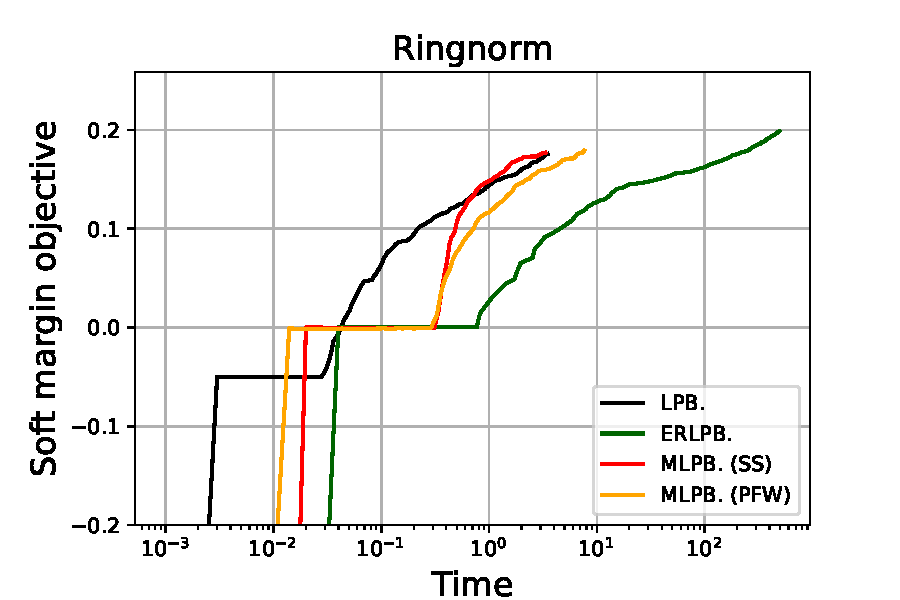
\includegraphics[keepaspectratio, scale=0.5]{figure/paper_curve.pdf}
        \end{minipage}
        &
        \begin{minipage}[t]{0.45\hsize}
            \centering
            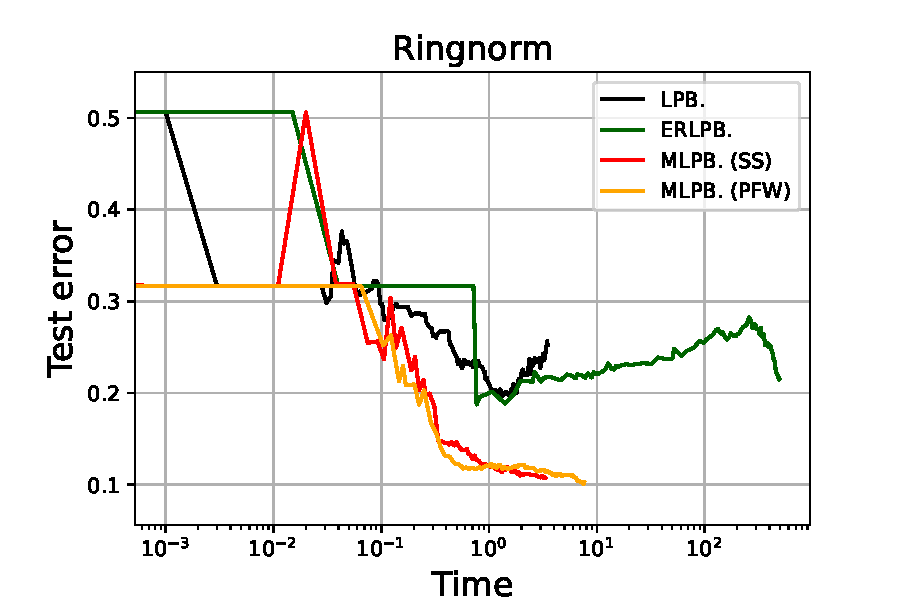
\includegraphics[keepaspectratio, scale=0.5]{figure/paper_test.pdf}
        \end{minipage}
    \end{tabular}
    \caption{%
        Comparison of the algorithm for the 0-th fold of %
        Ringnorm dataset with parameters $\epsilon = 0.01$ %
        and $\nu = 0.1m$. %
        \emph{Left:} %
        soft margin objective value vs. computation time (seconds). %
        \emph{Right:} %
        test error vs. computation time (seconds). %
    }
\end{figure}
We compare LPBoost, ERLPBoost, and our scheme 
on Gunnar R{\"{a}}tsch's benchmark dataset~\footnote{%
    Datasets are obtained from %
    \url{http://theoval.cmp.uea.ac.uk/~gcc/matlab/default.html\#benchmarks}. %
    \label{fnote:benchmark}%
}.
We use a server with 
Intel Xeon Gold 6124 CPU 2.60GHz processors. 
We call our scheme with secondary Algorithm~\ref{alg:lpb_subroutine} 
as MLPBoost. MLPB.~(SS) and MLPB.~(PFW) are MLPBoosts 
with FW algorithms~\ref{alg:ss_rule} and~\ref{alg:pairwise_rule}, 
respectively. 
The gradient boosting algorithms, 
like XGBoost~\citep{tianqi+:kdd16} or LightGBM~\citep{ke+:nips17}, 
solve different problems, 
so we do not compare our work to them. 
Note that the FW column corresponds to C-ERLPBoost. 

In order to solve the sub-problems of 
LPBoost, ERLPBoost, and MLPBoost, 
we use the Gurobi optimizer 9.0.1~\footnote{%
    We use the Gurobi optimizer. See %
    \url{https://www.gurobi.com/}. %
}. 
\paragraph{Settings.} 
We set the capping parameters 
$\nu \in N := \{pm \mid p = 0.1, 0.2, \dots, 0.5\}$ 
and the tolerance parameter $\epsilon = 0.01$, 
where $m$ is the number of training instances. 
We use the weak learner that 
returns the best decision tree of depth 2. 
\paragraph{Computation time.} 
We measure the CPU time and the System time using 
\texttt{/usr/bin/time -v} command. 
Some algorithms do not converge in a few days, 
so we abort the experiment by \texttt{timeout 20000s} command. 
We measure the running time with capping parameters 
over $N$ for each dataset and took their average. 
Table~\ref{table:time} shows the results.
The FW column is the FW algorithm with short-steps, 
and PFW is the Pairwise FW algorithm. 
As the table shows, MLPB.~(SS) and MLPB.~(PFW) terminates 
much faster than FW and PFW, respectively. 
These results indicate that 
LPBoost rule $\secalg$, shown in Algorithm~\ref{alg:lpb_subroutine}, 
significantly improves the objective. 
See the appendix for further comparisons. 
\begin{table}[h]
    \caption{ %
        Comparison of the computation time (seconds). %
        Each cell is the average computation time over %
        the capping parameters over $N$. %
        Some algorithm does not terminate in a few hours %
        so we abort them within some appropriate time. %
    }
    \label{table:time}
    \centering
    \begin{tabular}{lrrrrrrr}
    \toprule
            & \begin{tabular}{c} Shape \end{tabular} & \begin{tabular}{c} LPB. \end{tabular} & \begin{tabular}{c} ERLPB. \end{tabular} & \begin{tabular}{c} MLPB. \\ (SS only) \end{tabular} & \begin{tabular}{c} MLPB. \\ (PFW only) \end{tabular} & \begin{tabular}{c} MLPB. \\ (SS) \end{tabular} & \begin{tabular}{c} MLPB. \\ (PFW) \end{tabular}
 \\ \midrule \addlinespace[0.5em]
    Banana  &  $(5300, 3)$ &         $168.26$ &        $3434.75$ &          $>10^4$ &          $>10^4$ &        $1418.41$ &        $1398.68$
        \\ \addlinespace[0.5em]
    B.Cancer&  $(263, 10)$ &           $3.61$ &          $73.45$ &         $180.16$ &         $270.50$ &          $23.43$ &          $19.81$
        \\ \addlinespace[0.5em]
    Diabetes&   $(768, 9)$ &          $47.53$ &        $1478.77$ &          $>10^4$ &        $3471.77$ &         $201.46$ &         $270.51$
        \\ \addlinespace[0.5em]
    F.Solar &  $(144, 10)$ &           $2.30$ &           $2.46$ &          $13.34$ &          $80.73$ &          $31.64$ &          $46.45$
        \\ \addlinespace[0.5em]
    German  & $(1000, 21)$ &          $77.56$ &        $1391.91$ &          $>10^4$ &        $5692.32$ &         $181.43$ &         $201.88$
        \\ \addlinespace[0.5em]
    Heart   &  $(270, 14)$ &          $10.03$ &         $193.58$ &          $>10^3$ &         $183.09$ &          $44.11$ &          $24.26$
        \\ \addlinespace[0.5em]
    Image   & $(2086, 19)$ &           $8.25$ &         $107.52$ &          $>10^3$ &         $502.83$ &          $32.01$ &          $10.51$
        \\ \addlinespace[0.5em]
    R.norm  & $(7400, 21)$ &          $22.09$ &        $1148.16$ &          $>10^4$ &        $3350.87$ &          $26.76$ &          $36.73$
        \\ \addlinespace[0.5em]
    Splice  & $(2991, 61)$ &          $19.35$ &         $490.92$ &          $>10^4$ &         $943.98$ &         $122.08$ &          $37.88$
        \\ \addlinespace[0.5em]
    Thyroid &   $(215, 6)$ &           $0.70$ &           $0.66$ &         $367.51$ &           $0.35$ &           $2.71$ &           $0.61$
        \\ \addlinespace[0.5em]
    Titanic &    $(24, 4)$ &           $0.25$ &           $0.13$ &           $0.58$ &           $0.10$ &           $1.96$ &           $0.12$
        \\ \addlinespace[0.5em]
    Twonorm & $(7400, 21)$ &         $105.40$ &       $13031.38$ &          $>10^4$ &         $989.54$ &         $478.22$ &         $397.91$
        \\ \addlinespace[0.5em]
    Waveform& $(5000, 22)$ &         $437.29$ &        $9018.54$ &          $>10^4$ &          $>10^4$ &        $2243.07$ &        $1619.56$
        \\ \addlinespace[0.5em]
    \bottomrule
\end{tabular}
\end{table}
\paragraph{The worst case for LPBoost.} 
Although LPBoost outperforms the running time 
in Table~\ref{table:time}, 
it takes $m/2$ iterations for the worst case~\citep{warmuth+:nips07}. 
Even in this case, MLPBoost and ERLPBoost terminate in 2 iterations. 
\paragraph{Test errors.} 
For each dataset in the benchmark datasets, 
we first split them into train/test sets. 
Then, we perform the $5$-fold cross-validation over the training set, 
varying the capping parameter $\nu \in N$ to find the best one. 
Finally, train the algorithm using the whole training set 
with the best parameter and measure the test error with the test set. 
Table~\ref{table:cv5fold} summarizes the result. 
Since all the variants of MLPBoost solve the same problem, 
we only show MLPB.~(SS) for comparison. 
As the table shows, MLPBoosts achieve small test errors 
for most datasets. 
\begin{table}[h]
    \caption{%
        Test errors for $5$-fold cross validation %
        for the best parameters. 
    }
    \label{table:cv5fold}
    \bigskip
    \centering
    \begin{tabular}{lrrr}
    \toprule
	         &       LPB. &     ERLPB. & MLPB. (SS) \\ \midrule \addlinespace[0.5em]
	Banana   &       0.28 &       0.37 &       0.10 \\          \addlinespace[0.5em]
	B.Cancer &       0.40 &       0.49 &       0.28 \\          \addlinespace[0.5em]
	Diabetes &       0.26 &       0.26 &       0.24 \\          \addlinespace[0.5em]
	F.Solar  &       0.38 &       0.52 &       0.69 \\          \addlinespace[0.5em]
	German   &       0.28 &       0.35 &       0.27 \\          \addlinespace[0.5em]
	Heart    &       0.24 &       0.29 &       0.17 \\          \addlinespace[0.5em]
	Image    &       0.10 &       0.20 &       0.02 \\          \addlinespace[0.5em]
	Ringnorm &       0.18 &       0.18 &       0.03 \\          \addlinespace[0.5em]
	Splice   &       0.11 &       0.10 &       0.05 \\          \addlinespace[0.5em]
	Thyroid  &       0.09 &       0.05 &       0.05 \\          \addlinespace[0.5em]
	Titanic  &       0.60 &       0.60 &       0.60 \\          \addlinespace[0.5em]
	Twonorm  &       0.03 &       0.04 &       0.03 \\          \addlinespace[0.5em]
    \bottomrule
\end{tabular}
\end{table}


    
\section{Conclusion}
\label{sec_conclusions}

Our work consists of two studies that quantitatively and qualitatively investigate the influence of a CI service (e.g., \textsc{TravisCI}), and CI as a practice, on the time-to-delivery of merged PRs, respectively. In our quantitative study, we analyze 162,653 PRs of 87 GitHub projects to understand the factors that influence (and improve) the delivery time of merged PRs. In our qualitative study, we analyze 450 survey responses from participants of 73 projects (out of the initial 87 projects). We investigate the perceived influence of CI on the delivery time of merged PRs. We also study the perceived influence of CI on the code review and release processes.

As a key takeaway, our studies demonstrate that the adoption of \textsc{TravisCI}
will not necessarily deliver or merge PRs more quickly. Instead, the pivotal benefit of a CI service is to improve the mechanisms by which contributions to projects are processed (e.g., facilitating decisions on PR submissions), without compromising the quality of the project or overloading developers. The automation provided by CI and the boost in developers' confidence are key aspects of using CI. For instance, CI may help the process of sorting which PRs are worth reviewing (e.g., PRs with green builds).
Furthermore, open-source projects wishing to attract and retain external contributors should consider the use of CI in their pipeline, since CI is perceived to lower the contribution barrier while making contributors feel more confident and engaged in the project.

\section*{Acknowledgments}
\label{sec_Acknowledgments}

This work is partially supported by INES (\url{www.ines.org.br}), CNPq grants 465614/2014-0 and 425211/2018-5, CAPES grant 88887.136410/2017-00, FACEPE grants APQ-0399-1.03/17, and PRONEX APQ/0388-1.03/14.

\section*{Data Availability}
For replication purposes, we publicize our datasets and results to the interested researcher: \url{https://prdeliverydelay.github.io/#datasets}

\section*{Declarations}

\textbf{Conflict of interests}. The authors declare that they have no conflict of interest.


    \bibliographystyle{unsrtnat}
    \bibliography{mitsuboshi}

    \appendix
    \section{Technical lemmas and proofs}
\label{appendix:technical_lem.}
The following lemma shows the maximum value of the relative entropy 
from the uniform distribution 
over the capped probability simplex $\psimplex{m}_{\nu}$.
\begin{lem.}
    \label{lem:relative_entropy_bound}
    $
        \max_{\bm{d} \in \psimplex{m}_{\nu}}
        \Delta(\bm{d}) \leq \ln \frac{m}{\nu}
    $.
\end{lem.}
\begin{proof}
    Since the relative entropy from the uniform distribution 
    achieves its maximal value 
    at the extreme points of $\psimplex{m}_{\nu}$, 
    a maximizer has the form 
    \begin{align}
        \nonumber
        \bm{d} = (
            \underbrace{1/\nu, 1/\nu, \dots, 1/\nu}_{k \text{ elements}},
            s,
            0, 0, \dots, 0
        ),
        \quad s = 1 - \frac{k}{\nu} \leq \frac 1 \nu
    \end{align}
    for some $k \in [m]$. 
    Plugging the maximizer into $\Delta(\bm{d})$, 
    we can write the objective function as 
    $\Delta(\bm{d}) = (k/\nu) \ln (m/\nu) + s \ln (sm)$. 
    If $s = 0$, $\Delta(\bm{d}) = \ln (m/\nu)$ holds since $k = \nu$. 
    If $s > 0$, $k / \nu < 1$ so that 
    \begin{align*}
        \Delta(\bm{d}) \leq \frac k \nu \ln \frac m \nu
            + \left(1 - \frac k \nu\right) \ln \frac m \nu
            = \ln \frac m \nu.
    \end{align*}
\end{proof}
Therefore, by setting $\eta = \frac{2}{\epsilon} \ln \frac{m}{\nu}$, 
the entropy term does not exceed $\frac{\epsilon}{2}$. 

The following lemma shows the dual problem of the edge minimization. 
\begin{lem.}
    \label{lem:dual_problem}
    Let $f : \mathbb R^m \to \{0, +\infty\}$, 
    $g : \mathbb R^n \to \mathbb R$ be 
    functions defined as 
    \begin{align}
        \nonumber
        f(\bm{d}) =
        \begin{cases}
                  0 & \bm{d} \in    \psimplex{m}_{\nu} \\
            +\infty & \bm{d} \notin \psimplex{m}_{\nu}
        \end{cases},
        \qquad \qquad \qquad
        g(\bm{\theta}) = \max_{j \in [n]} \theta_j.
    \end{align}
    Then, the dual problem of edge minimization 
    % $\min_{\bm{d}} f(\bm{d}) + g(A^\top \bm{d})$ is
    % $\max_{\bm{w} \in \Delta_n} - f^\star(A\bm{w})$.
    \begin{align}
        \label{eq:appendix_edge_minimization}
        \min_{\bm{d}} f(\bm{d}) + g(A^\top \bm{d})
    \end{align}
    is the soft margin maximization 
    \begin{align}
        \label{eq:appendix_smm}
        \max_{\bm{w} \in \psimplex{n}} - f^\star( -A \bm{w} ).
    \end{align}
    Further, the strong duality holds. 
\end{lem.}
\begin{proof}
    We can use Theorem~\ref{thm:strong_duality} to derive the dual problem. 
    Since 
    \begin{align*}
        \bm{g}^\star(\bm{w}) = 
        \begin{cases}
                  0 & \bm{w} \in    \psimplex{n} \\
            +\infty & \bm{w} \notin \psimplex{n}
        \end{cases},
    \end{align*}
    one can verify the dual form is given as~(\ref{eq:appendix_smm}). 
    To prove the strong duality, 
    it is enough to prove 
    $
        \bm{0} \in \interior\left(
            \domain g - A^\top \domain f
        \right)
    $. 
    By definition, $\domain g = \mathbb R^n$ and 
    $\domain f = \psimplex{m}_{\nu}$ and hence 
    \begin{align*}
        \domain g - A^\top \domain f
        = \left\{
            \bm{w} - A^\top \bm{d} \mid
            \bm{w} \in \mathbb{R}^n, \bm{d} \in \psimplex{m}_{\nu}
        \right\}.
    \end{align*}
    Obviously, $\bm{0} \in \interior (\domain g - A^\top \domain f)$ 
    and thus the strong duality holds. 
\end{proof}
Since 
\begin{align*}
    f^\star(-A\bm{w}) 
    = \sup_{\bm{d}} \left[ - \bm{d}^\top A \bm{w} - f(\bm{d}) \right]
    = \max_{\bm{d} \in \psimplex{m}_{\nu}} - \bm{d}^\top A \bm{w}
    = \min_{\bm{d} \in \psimplex{m}_{\nu}} \bm{d}^\top A \bm{w},
\end{align*}
we can write the dual problem~(\ref{eq:appendix_smm}) explicitly:
\begin{align*}
    \max_{\bm{w} \in \psimplex{n}} - f^\star ( -A \bm{w} )
        = - \min_{\bm{w} \in \psimplex{n}}
            \max_{\bm{d} \in \psimplex{m}_{\nu}}
        \bm{d}^\top A \bm{w}.
\end{align*}
% By the same derivation, we get the dual problem 
% for the regularized edge minimization problem. 
We get the dual problem for the regularized edge minimization problem 
by a similar derivation. 
\begin{cor.}
    \label{lem:smoothed_dual_problem}
    Let $f, g$ be the functions defined in Lemma~\ref{lem:dual_problem} and 
    let $\Delta(\bm{d}) = \sum_{i=1}^m d_i \ln d_i + \ln(m)$ be 
    the relative entropy function from the uniform distribution. 
    Define $\tilde{f} = f + (1/\eta) \Delta$ for some $\eta > 0$. 
    Then, the dual problem of 
    \begin{align}
        \nonumber
        \min_{\bm{d}} \tilde{f}(\bm{d}) + g(A^\top \bm{d})
        \qquad \text{ is } \qquad
        \max_{\bm{w} \in \psimplex{n}} - \tilde{f}^\star(-A \bm{w}).
    \end{align}
\end{cor.}

\subsection{Proof of Lemma~\ref{lem:fenchel_conjugate_functions}}
\begin{proof}
    By the definition of Fenchel conjugate, 
    \begin{align*}
        \tilde{f}^\star(\bm{\theta})
        & = \sup_{\bm{d}} \left\{
            \bm{d}^\top \bm{\theta} - \tilde{f}(\bm{d})
        \right\}
        \geq \sup_{\bm{d}} \left\{
            \bm{d}^\top \bm{\theta} - f(\bm{d}) - c
        \right\}
        = f^\star(\bm{\theta}) - c, \\
        \tilde{f}^\star(\bm{\theta})
        & = \sup_{\bm{d}} \left\{
            \bm{d}^\top \bm{\theta} - \tilde{f}(\bm{d})
        \right\}
        \leq \sup_{\bm{d}} \left\{
            \bm{d}^\top \bm{\theta} - f(\bm{d})
        \right\}
        = f^\star(\bm{\theta}).
    \end{align*}
\end{proof}
By Lemma~\ref{lem:relative_entropy_bound} 
and~\ref{lem:fenchel_conjugate_functions}, 
we get 
$
    \tilde{f}^\star (-A\bm{w}) - \frac{\epsilon}{2}
    \leq f(-A\bm{w}) \leq \tilde{f}^\star(-A\bm{w})
$ for all $-A \bm{w}$ 
if $\eta \geq \frac{2}{\epsilon} \ln \frac{m}{\nu}$. 


\subsection{
    Proof of Theorem~\ref{thm:mlpboost_convergence_guarantee}
    for the short-step FW rule~\ref{alg:ss_rule}
}
Recall that in the proof of Theorem~\ref{thm:mlpboost_convergence_guarantee}, 
we showed the inequality 
$\epsilon_t - \epsilon_{t+1} \geq \frac{1}{8 \eta} \epsilon_t^2$ 
for the short-step case. 
We prove $\epsilon_t \leq \frac{8\eta}{t + 2}$ by induction on $t$. 
For the base case, $t = 1$, by Lemma~\ref{lem:fenchel_conjugate_functions}, 
\begin{align*}
    \epsilon_1
    = \min_{\tau \in \{0, 1\}} (\bm{d}_\tau^\top A)_{j_{\tau + 1}}
        + \tilde{f}^\star (- A\bm{w}_1)
    \leq 1 + f^\star (- A\bm{w}_1)
    \leq 2
    \leq \frac{8\eta}{1 + 2}.
\end{align*}
For the inductive case, assume that $\epsilon_t \leq \frac{8\eta}{t+2}$ 
for $t \geq 1$. 
By the inequality
$\epsilon_t - \epsilon_{t+1} \geq \frac{1}{8 \eta} \epsilon_t^2$, 
we have
\begin{align}
    \label{eq:appendix_shortstep_01}
    \epsilon_{t+1} 
    \leq \left(1 - \frac{1}{8\eta} \epsilon_t\right) \epsilon_t.
\end{align}
By simple calculation, 
one can see that the maximizer $\epsilon$ of the RHS over $\mathbb{R}$ is 
$\epsilon = 4\eta$. 
By the inductive assumption, $\epsilon_t \leq \frac{8 \eta}{t + 2}$. 
Since $\frac{8\eta}{t+2}$ is 
the maximizer of~(\ref{eq:appendix_shortstep_01}) 
over $[0, \frac{8\eta}{t+2}]$, 
we can plug this value into~(\ref{eq:appendix_shortstep_01}). 
\begin{align*}
    \epsilon_{t+1} 
    \leq \left(1 - \frac{1}{8\eta} \frac{8\eta}{t+2}\right)
    \frac{8\eta}{t+2}
    = \frac{t+1}{t+2} \frac{8\eta}{t+2}
    \leq \frac{8\eta}{t+3}
\end{align*}
Therefore, $\epsilon_{t} \leq \frac{8\eta}{t+2}$ holds for all $t \geq 1$. 
Thus, we obtain the desired result. 

    \section{Additional experiments}
\label{sec:appendix_experiemnt}
This section includes experiments, not in the main paper. 
We first show the comparison of boosting algorithms, 
LPBoost, ERLPBoost, C-ERLPBoost, and our scheme. 
Since C-ERLPBoost is an instance of the short-step FW algorithm, 
we call it FW. 
We call our scheme with secondary algorithm~\ref{alg:lpb_subroutine} 
as MLPBoost. 
Figure~\ref{fig:appendix_margin_objectives} shows the convergence curve. 
MLPB.~(SS) is MLPBoost with FW algorithm~\ref{alg:ss_rule}, 
and MLPB.~(PFW) is MLPBoost 
with Pairwise FW algorithm~\ref{alg:pairwise_rule}. 
As expected, our algorithm converges faster than ERLPBoost 
and is competitive with LPBoost. 
\begin{figure}[p]
    \centering
    \begin{tabular}{ccc}
        \begin{minipage}[t]{0.31\hsize}
            \centering
            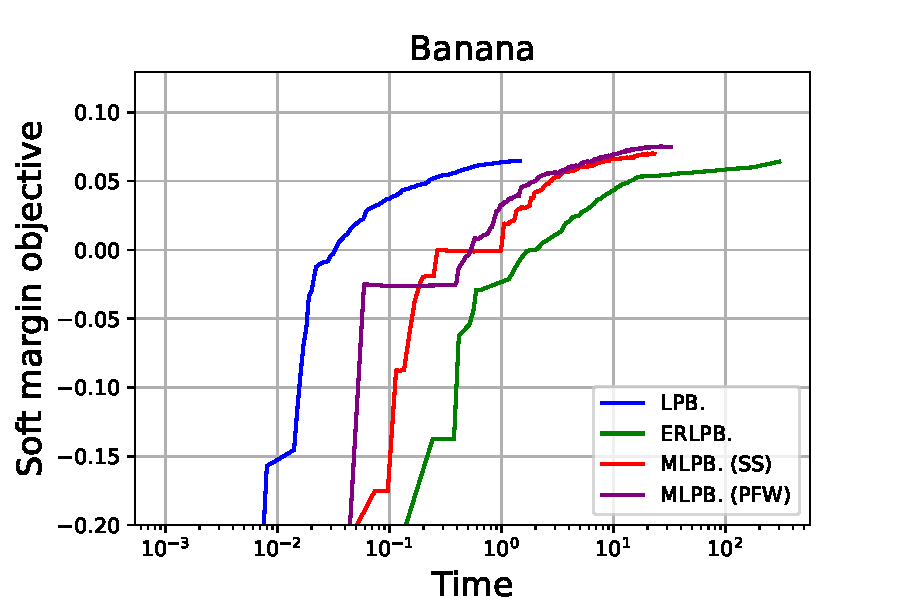
\includegraphics[keepaspectratio, scale=0.30]
            {figure/curve_logtime_banana.pdf}
        \end{minipage}
        &
        \begin{minipage}[t]{0.31\hsize}
            \centering
            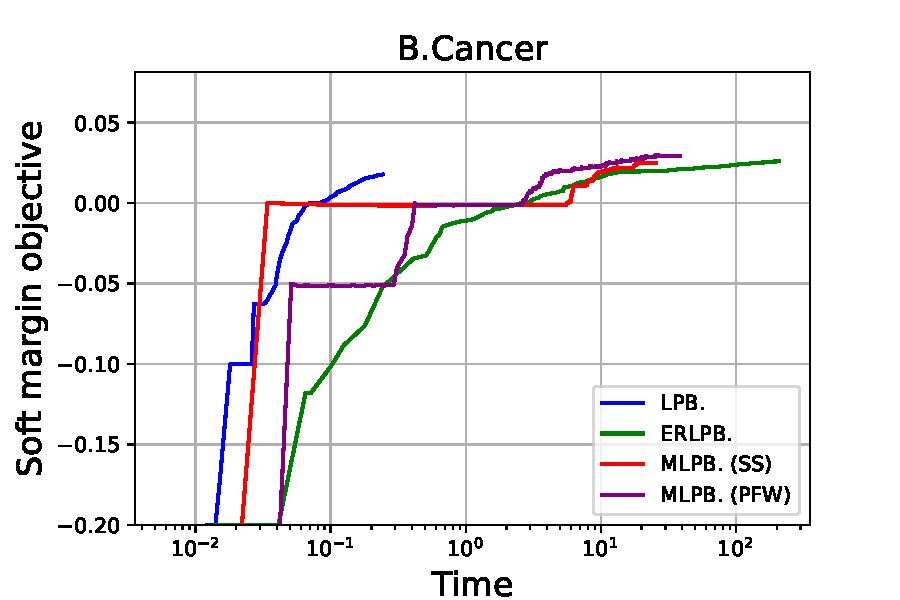
\includegraphics[keepaspectratio, scale=0.30]
            {figure/curve_logtime_breast_cancer.pdf}
        \end{minipage}
        &
        \begin{minipage}[t]{0.31\hsize}
            \centering
            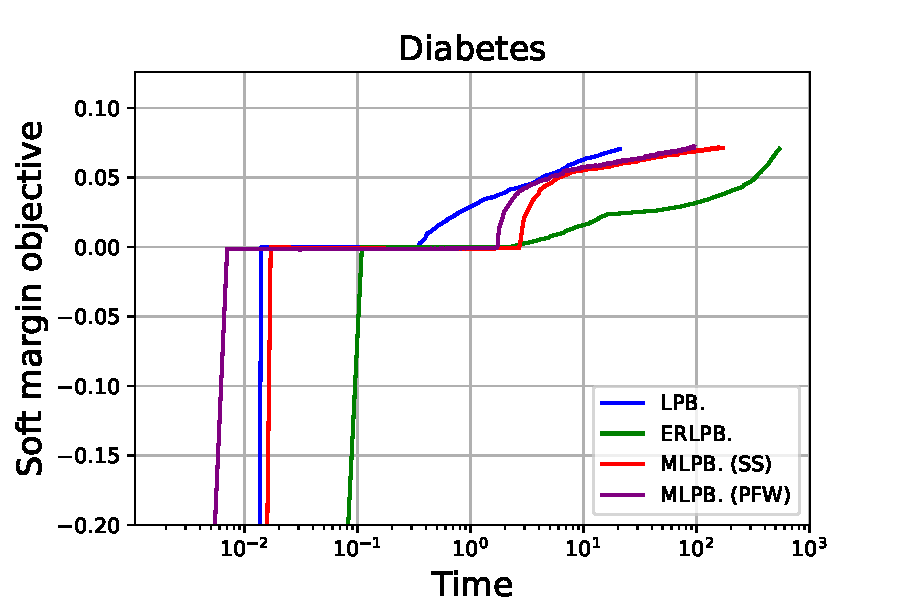
\includegraphics[keepaspectratio, scale=0.30]
            {figure/curve_logtime_diabetis.pdf}
        \end{minipage}
        \\
        \begin{minipage}[t]{0.31\hsize}
            \centering
            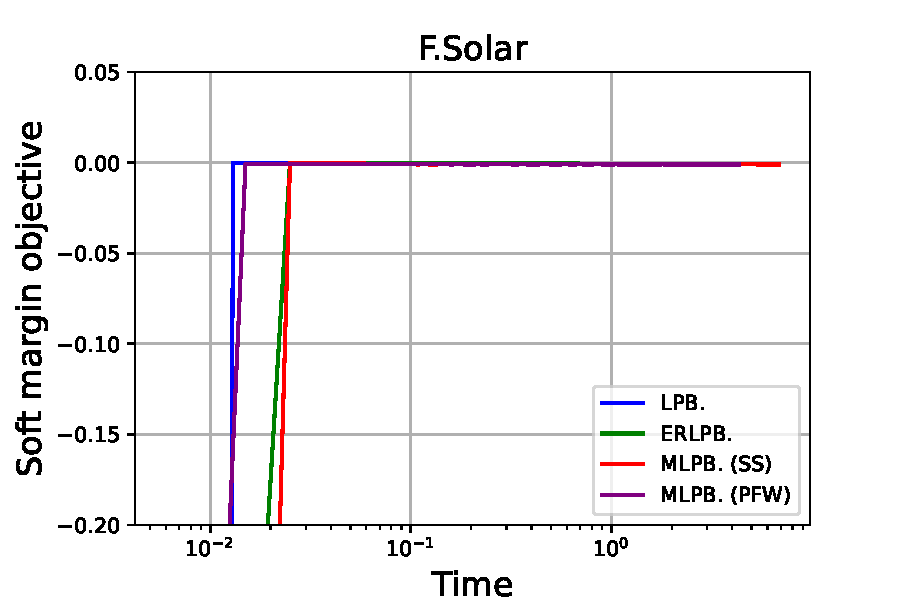
\includegraphics[keepaspectratio, scale=0.30]
            {figure/curve_logtime_flare_solar.pdf}
        \end{minipage}
        &
        \begin{minipage}[t]{0.31\hsize}
            \centering
            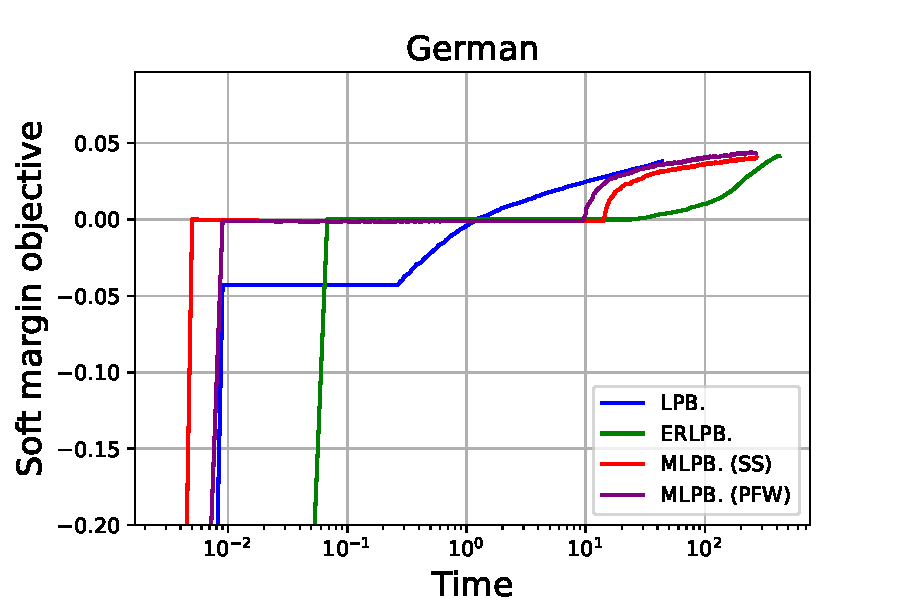
\includegraphics[keepaspectratio, scale=0.30]
            {figure/curve_logtime_german.pdf}
        \end{minipage}
        &
        \begin{minipage}[t]{0.31\hsize}
            \centering
            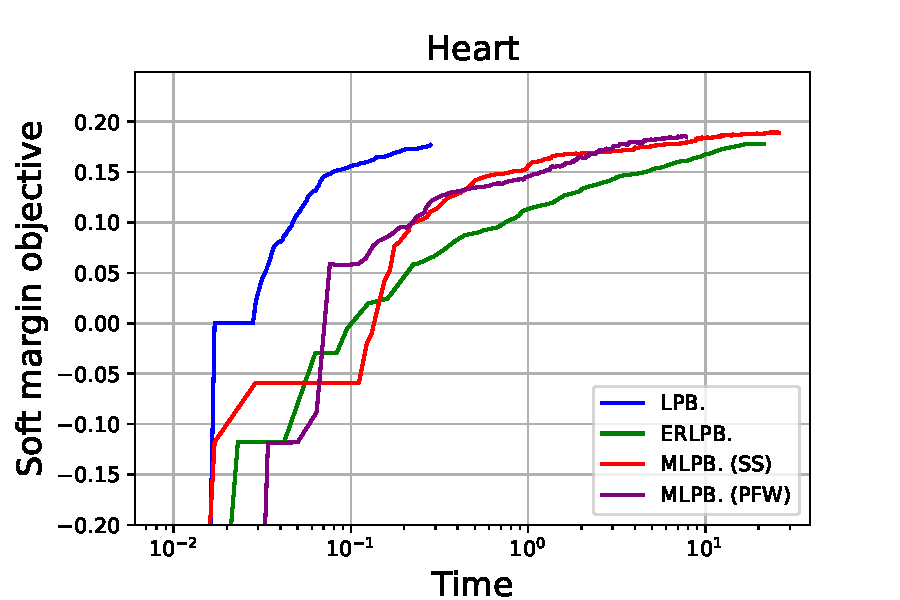
\includegraphics[keepaspectratio, scale=0.30]
            {figure/curve_logtime_heart.pdf}
        \end{minipage}
        \\
        \begin{minipage}[t]{0.31\hsize}
            \centering
            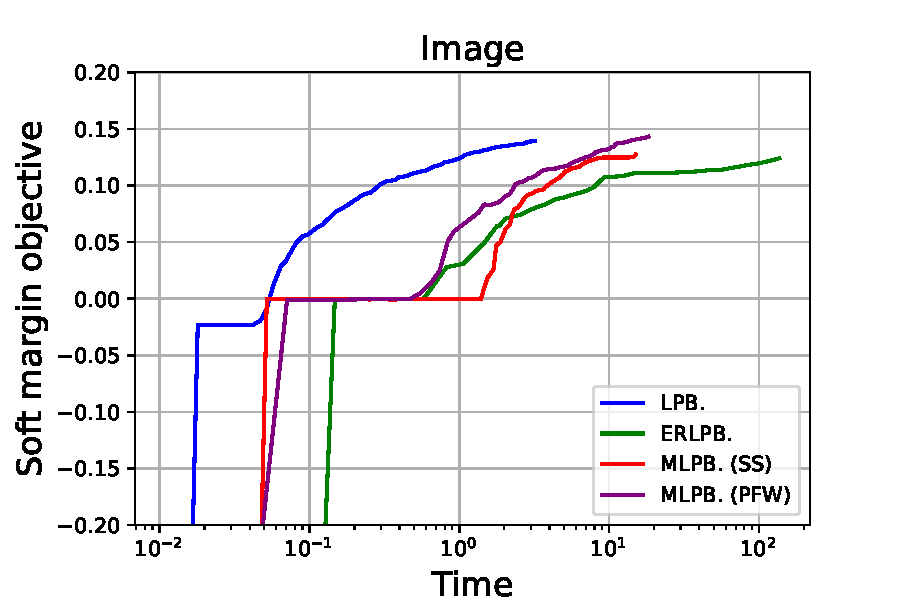
\includegraphics[keepaspectratio, scale=0.30]
            {figure/curve_logtime_image.pdf}
        \end{minipage}
        &
        \begin{minipage}[t]{0.31\hsize}
            \centering
            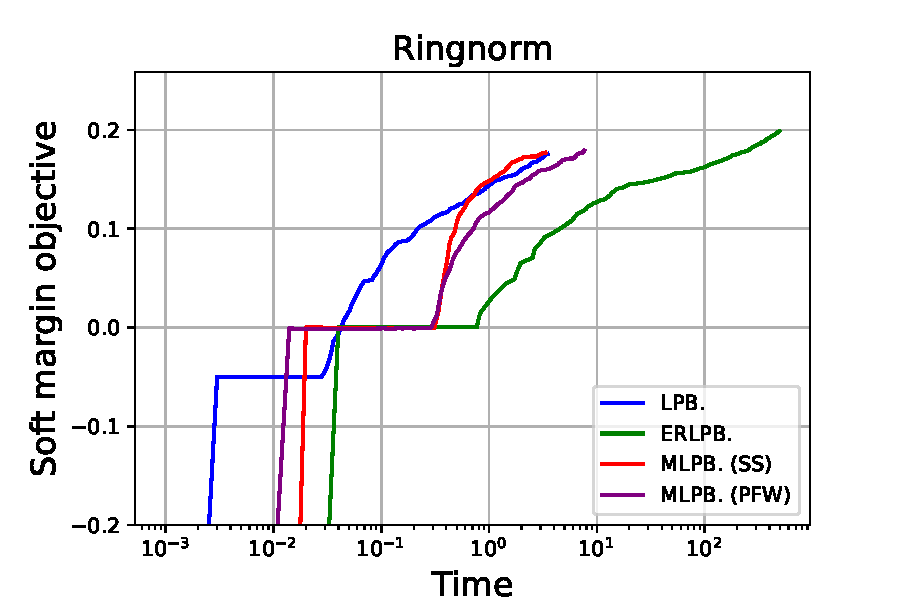
\includegraphics[keepaspectratio, scale=0.30]
            {figure/curve_logtime_ringnorm.pdf}
        \end{minipage}
        &
        \begin{minipage}[t]{0.31\hsize}
            \centering
            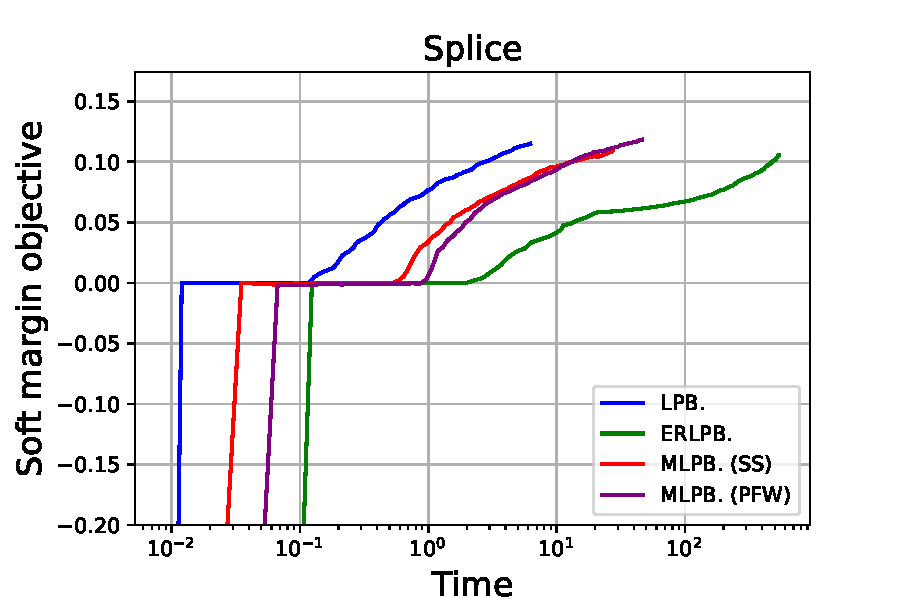
\includegraphics[keepaspectratio, scale=0.30]
            {figure/curve_logtime_splice.pdf}
        \end{minipage}
        \\
        \begin{minipage}[t]{0.31\hsize}
            \centering
            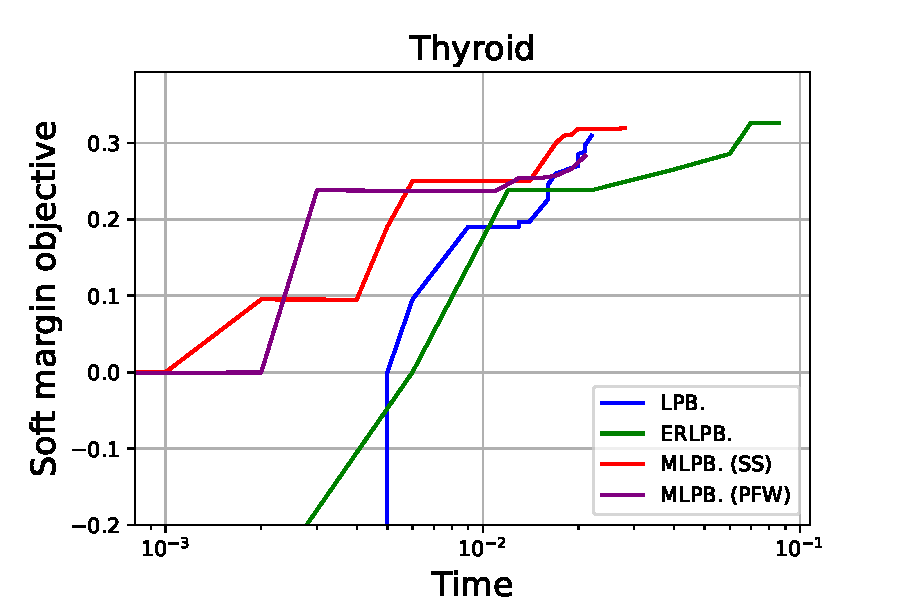
\includegraphics[keepaspectratio, scale=0.30]
            {figure/curve_logtime_thyroid.pdf}
        \end{minipage}
        &
        \begin{minipage}[t]{0.31\hsize}
            \centering
            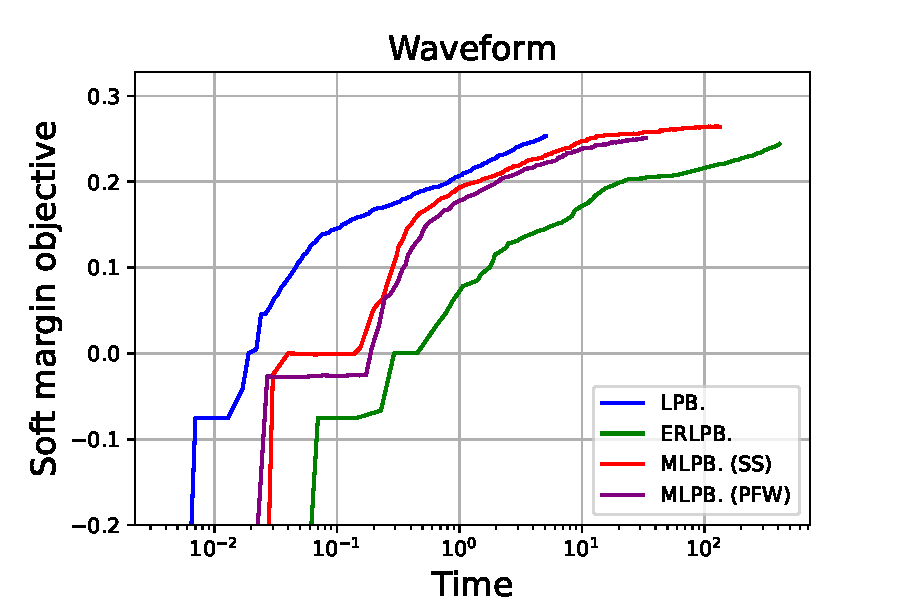
\includegraphics[keepaspectratio, scale=0.30]
            {figure/curve_logtime_waveform.pdf}
        \end{minipage}
        &
        \begin{minipage}[t]{0.31\hsize}
            \centering
            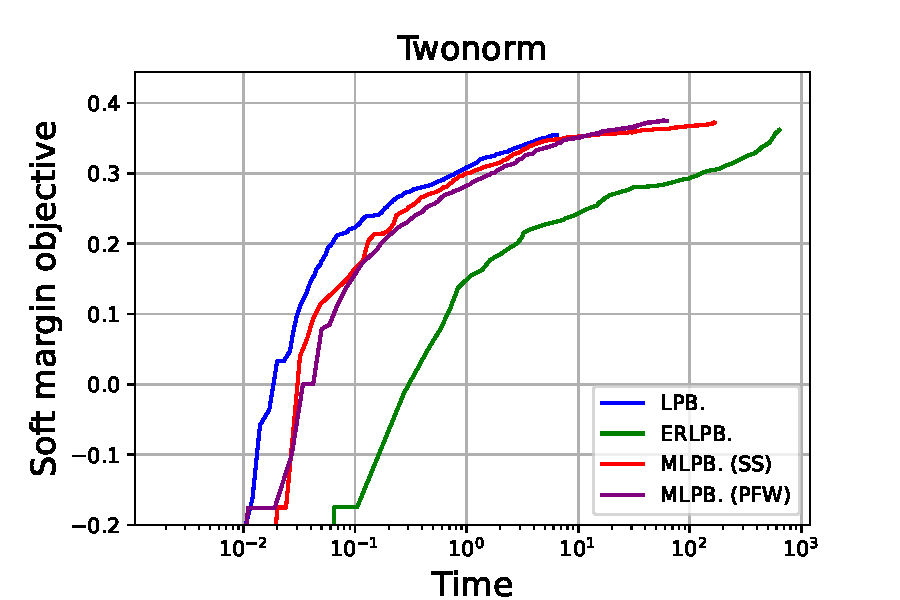
\includegraphics[keepaspectratio, scale=0.30]
            {figure/curve_logtime_twonorm.pdf}
        \end{minipage}
    \end{tabular}
    \caption{%
        Time vs. soft margin objective %
        with parameters $\nu = 0.1m$ and $\epsilon = 0.01$. %
        Note that the time axis is log-scale. %
        For many datasets, MLPBoosts tend to achieve %
        a large margin rapidly. %
    }
    \label{fig:appendix_margin_objectives}
\end{figure}

Further, we compare the test error decrease. 
Figure~\ref{fig:appendix_test_errors} shows the test error curves. 
MLPB.~(SS) achieves low test errors in most datasets. 
\begin{figure}[p]
    \centering
    \begin{tabular}{ccc}
        \begin{minipage}[t]{0.31\hsize}
            \centering
            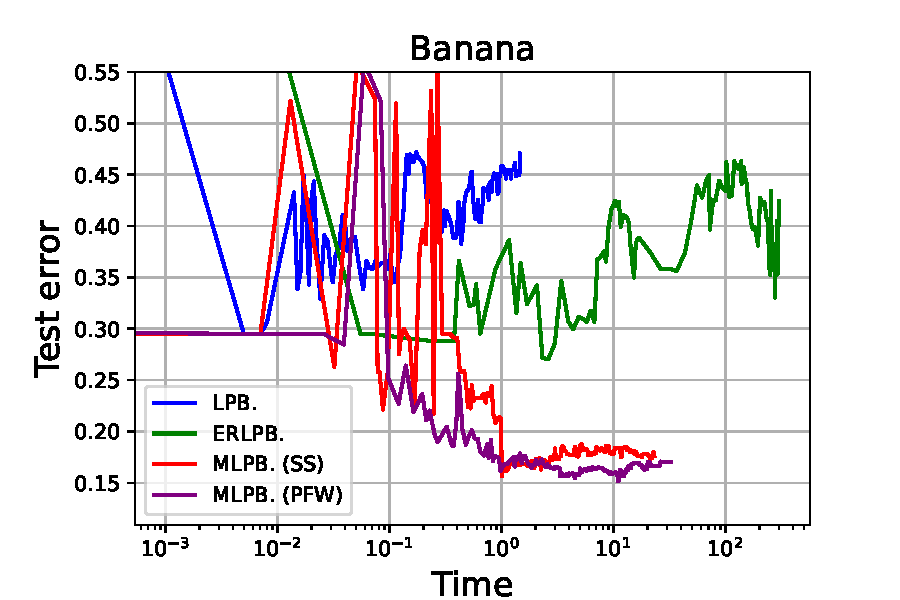
\includegraphics[keepaspectratio, scale=0.30]
            {figure/test_logtime_banana.pdf}
        \end{minipage}
        &
        \begin{minipage}[t]{0.31\hsize}
            \centering
            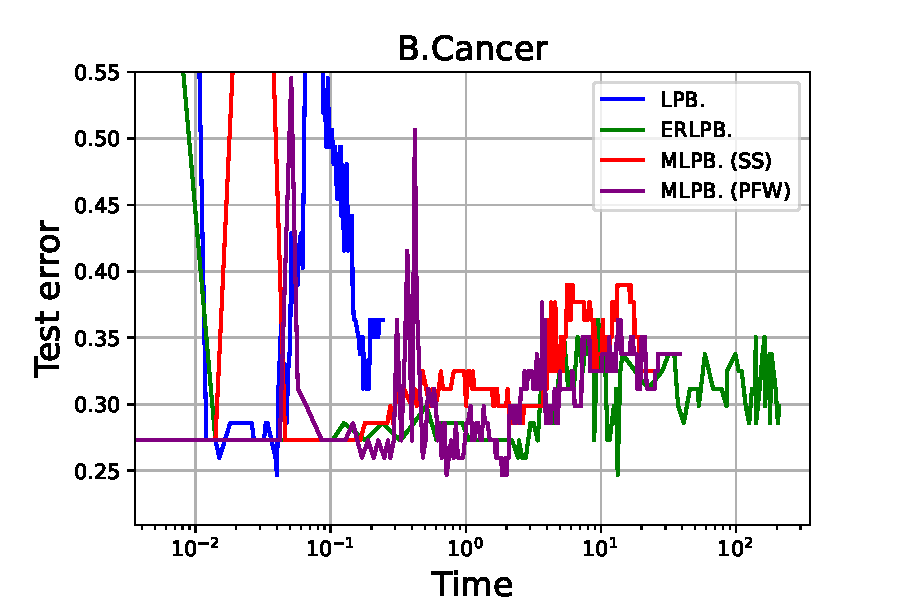
\includegraphics[keepaspectratio, scale=0.30]
            {figure/test_logtime_breast_cancer.pdf}
        \end{minipage}
        &
        \begin{minipage}[t]{0.31\hsize}
            \centering
            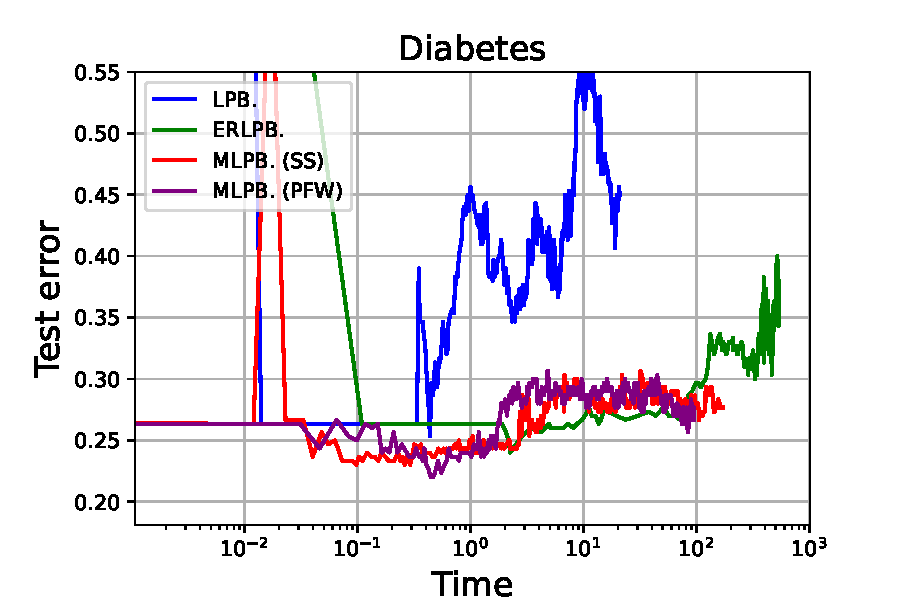
\includegraphics[keepaspectratio, scale=0.30]
            {figure/test_logtime_diabetis.pdf}
        \end{minipage}
        \\
        \begin{minipage}[t]{0.31\hsize}
            \centering
            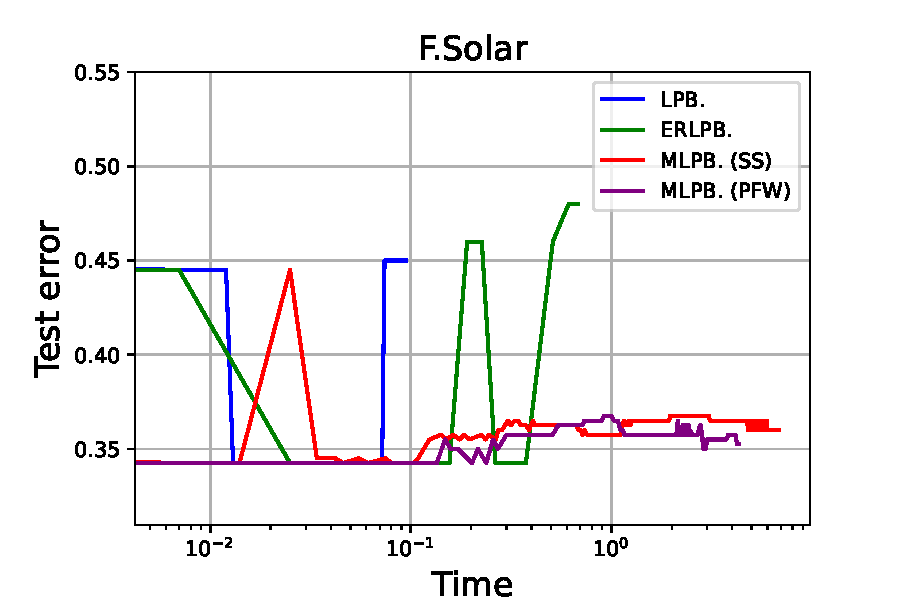
\includegraphics[keepaspectratio, scale=0.30]
            {figure/test_logtime_flare_solar.pdf}
        \end{minipage}
        &
        \begin{minipage}[t]{0.31\hsize}
            \centering
            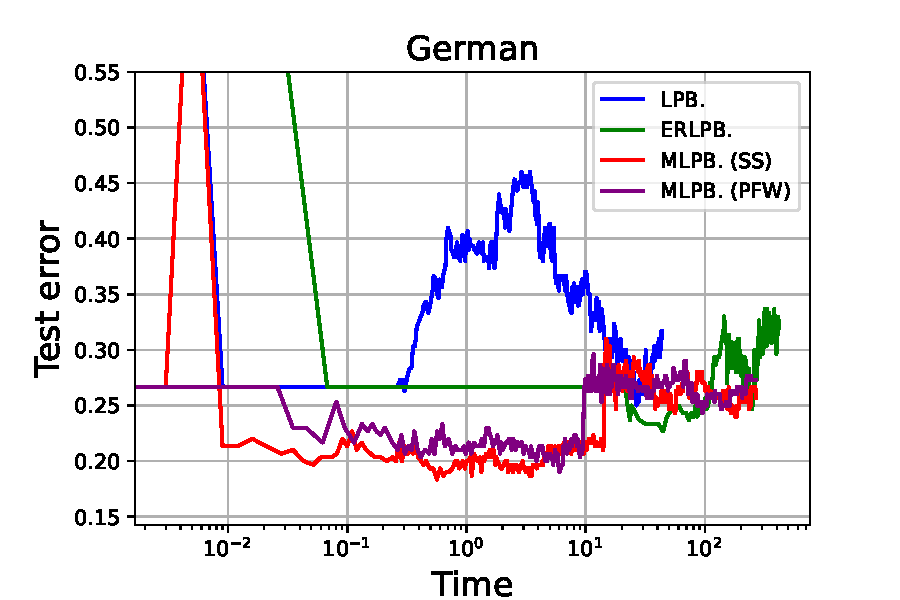
\includegraphics[keepaspectratio, scale=0.30]
            {figure/test_logtime_german.pdf}
        \end{minipage}
        &
        \begin{minipage}[t]{0.31\hsize}
            \centering
            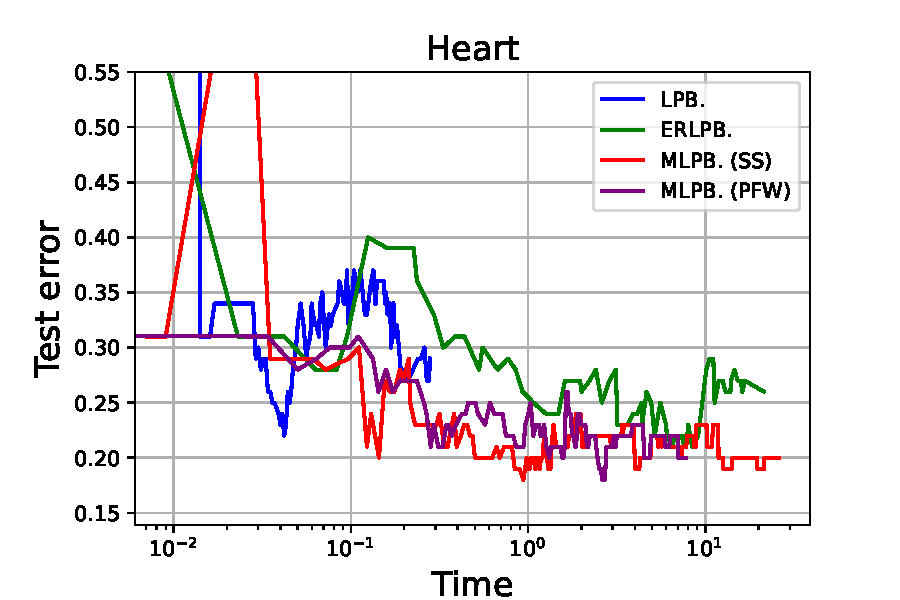
\includegraphics[keepaspectratio, scale=0.30]
            {figure/test_logtime_heart.pdf}
        \end{minipage}
        \\
        \begin{minipage}[t]{0.31\hsize}
            \centering
            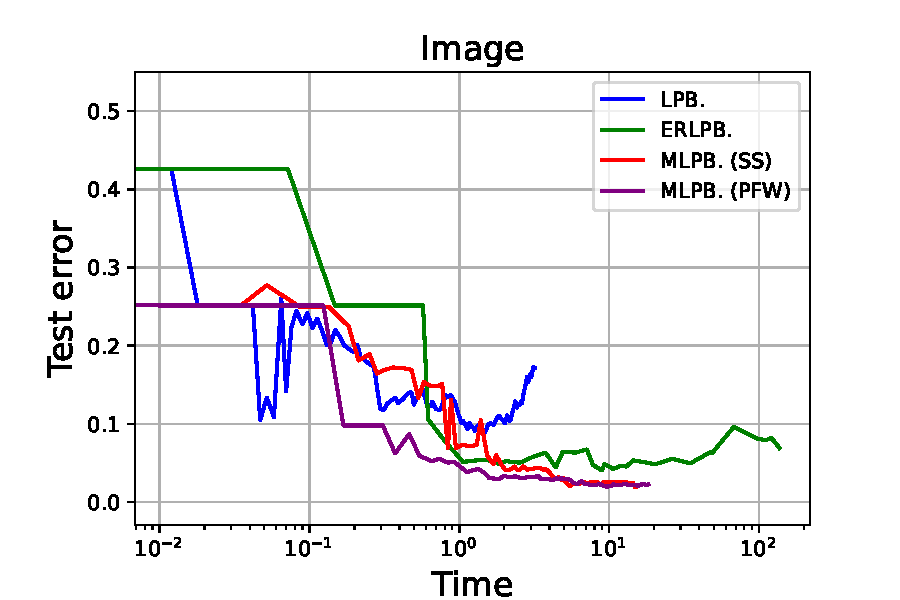
\includegraphics[keepaspectratio, scale=0.30]
            {figure/test_logtime_image.pdf}
        \end{minipage}
        &
        \begin{minipage}[t]{0.31\hsize}
            \centering
            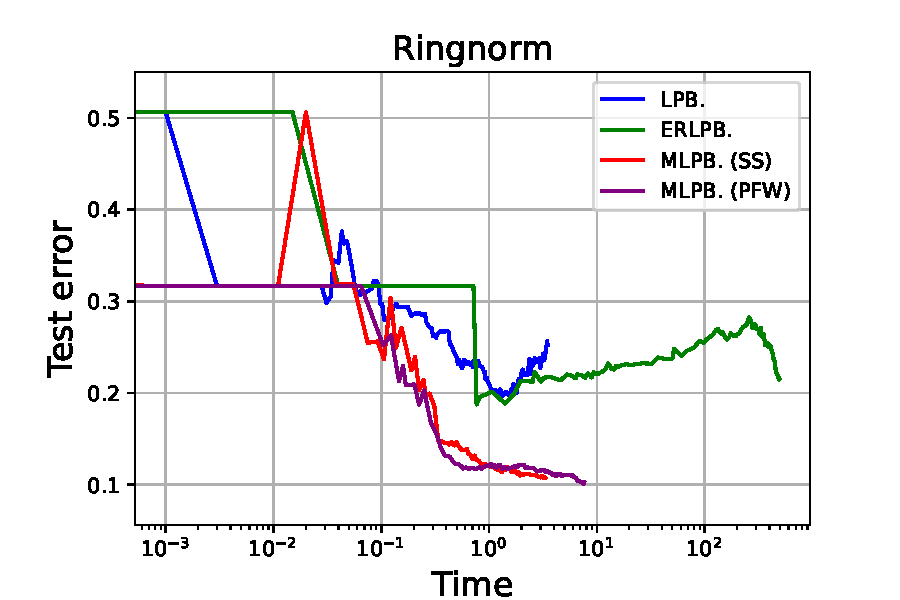
\includegraphics[keepaspectratio, scale=0.30]
            {figure/test_logtime_ringnorm.pdf}
        \end{minipage}
        &
        \begin{minipage}[t]{0.31\hsize}
            \centering
            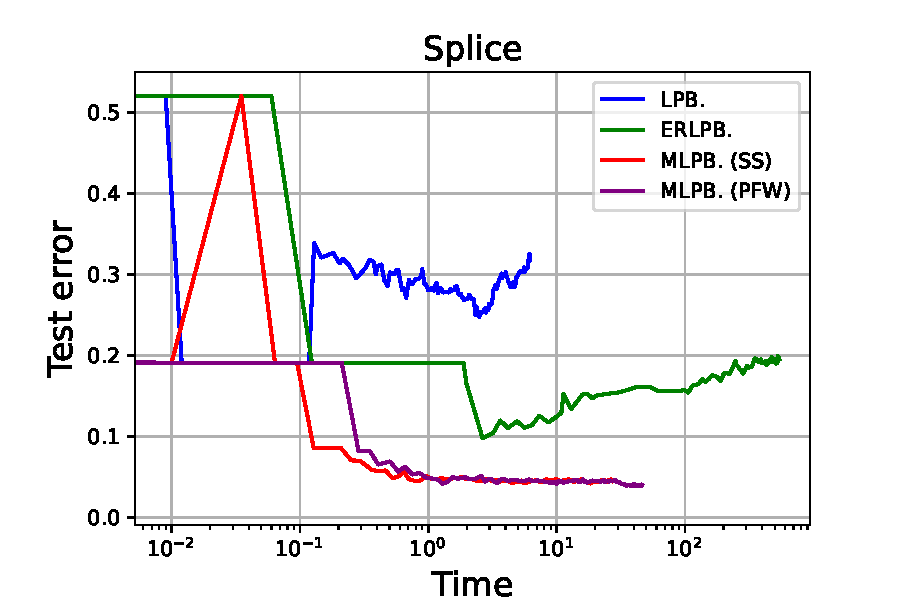
\includegraphics[keepaspectratio, scale=0.30]
            {figure/test_logtime_splice.pdf}
        \end{minipage}
        \\
        \begin{minipage}[t]{0.31\hsize}
            \centering
            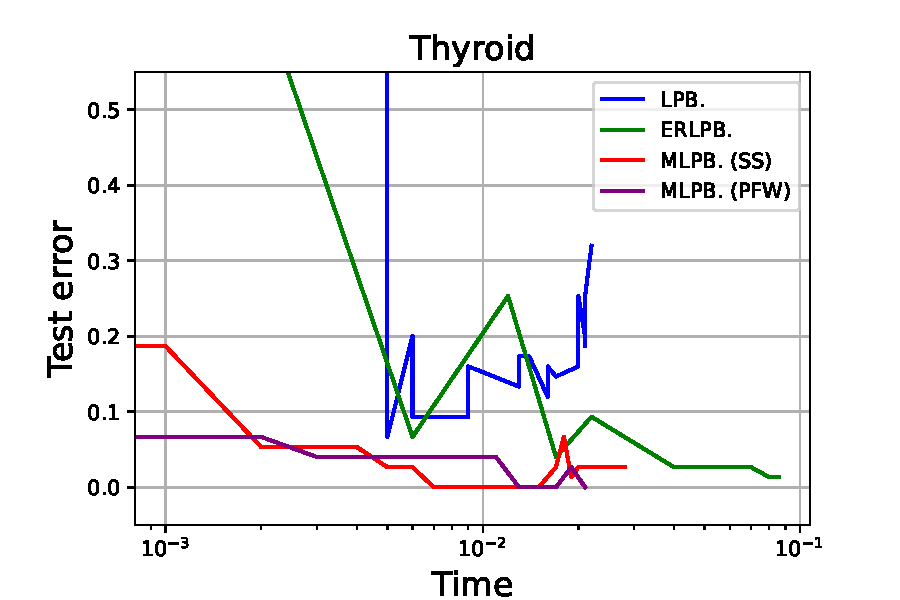
\includegraphics[keepaspectratio, scale=0.30]
            {figure/test_logtime_thyroid.pdf}
        \end{minipage}
        &
        \begin{minipage}[t]{0.31\hsize}
            \centering
            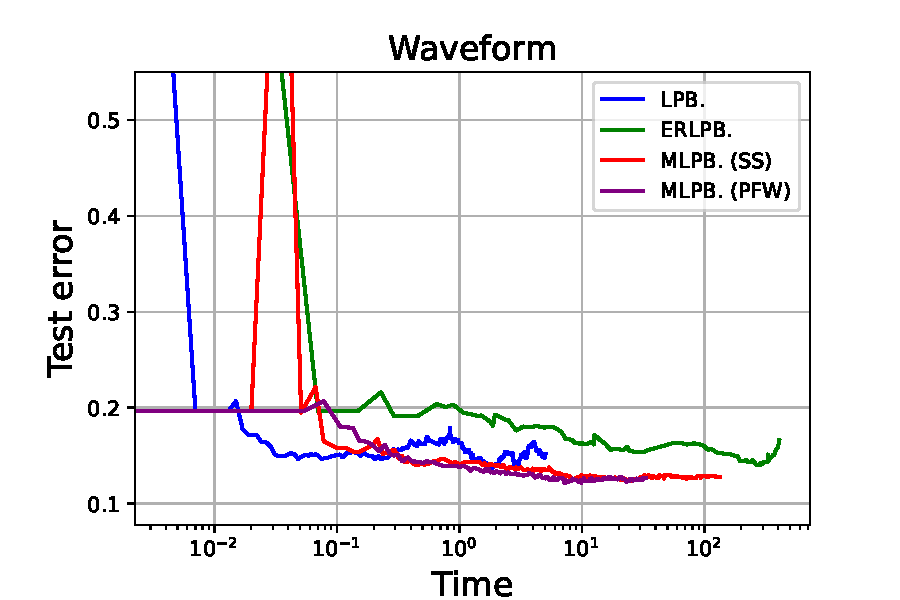
\includegraphics[keepaspectratio, scale=0.30]
            {figure/test_logtime_waveform.pdf}
        \end{minipage}
        &
        \begin{minipage}[t]{0.31\hsize}
            \centering
            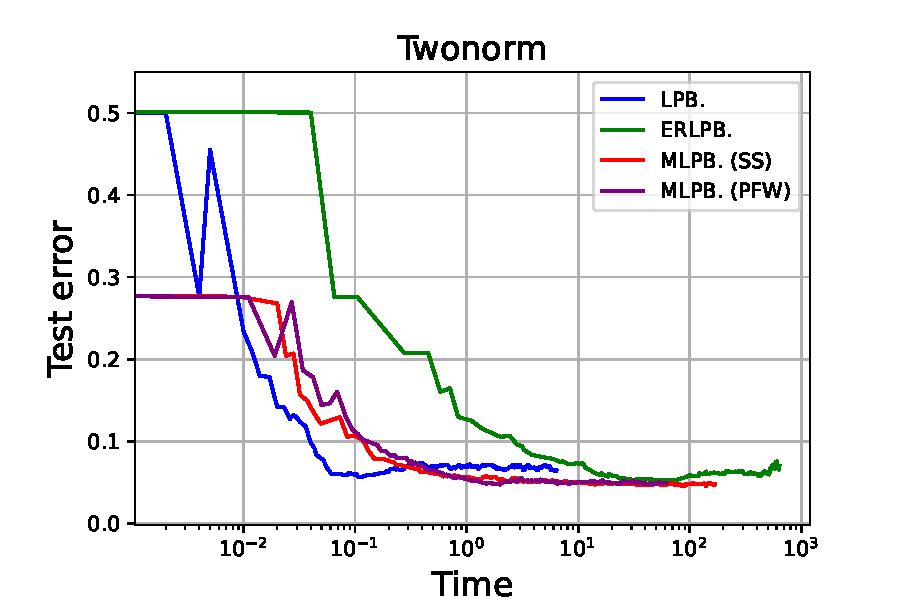
\includegraphics[keepaspectratio, scale=0.30]
            {figure/test_logtime_twonorm.pdf}
        \end{minipage}
    \end{tabular}
    \caption{%
        Time vs. test errors for the 0th fold of each dataset %
        with parameters $\nu = 0.1m$ and $\epsilon = 0.01$. %
        Note that the time axis is log-scale. %
        For many datasets, MLPBoost tends to decrease %
        the test error. %
    }
    \label{fig:appendix_test_errors}
\end{figure}

Now, we compare MLPBoosts to the Frank-Wolfe algorithms, FW and PFW. 
Figure~\ref{fig:appendix_lpbcall} shows 
the number of $\secalg$ updates. 
This figure shows that 
the secondary update $\secalg$ yields better progress 
in early iterations. In the latter half, 
$\fwalg$ yields better progress. 
\begin{figure}[p]
    \centering
    \begin{tabular}{ccc}
        \begin{minipage}[t]{0.31\hsize}
            \centering
            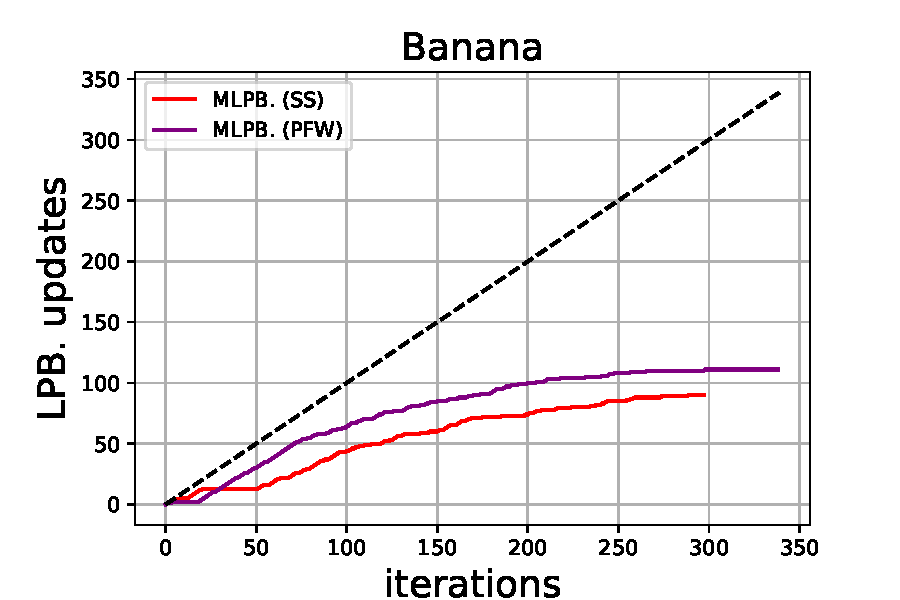
\includegraphics[keepaspectratio, scale=0.30]
            {figure/mlpb_lpb_update_banana.pdf}
        \end{minipage}
        &
        \begin{minipage}[t]{0.31\hsize}
            \centering
            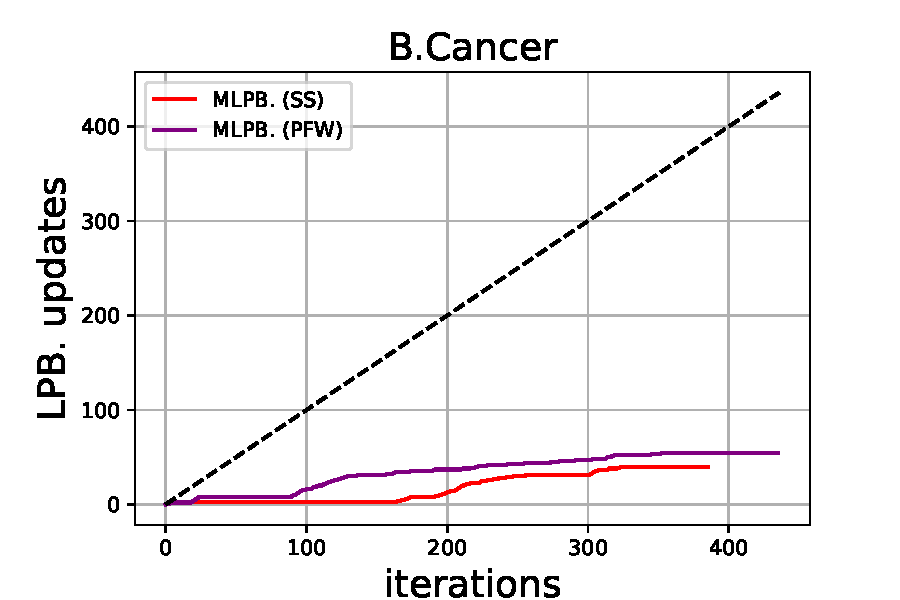
\includegraphics[keepaspectratio, scale=0.30]
            {figure/mlpb_lpb_update_breast_cancer.pdf}
        \end{minipage}
        &
        \begin{minipage}[t]{0.31\hsize}
            \centering
            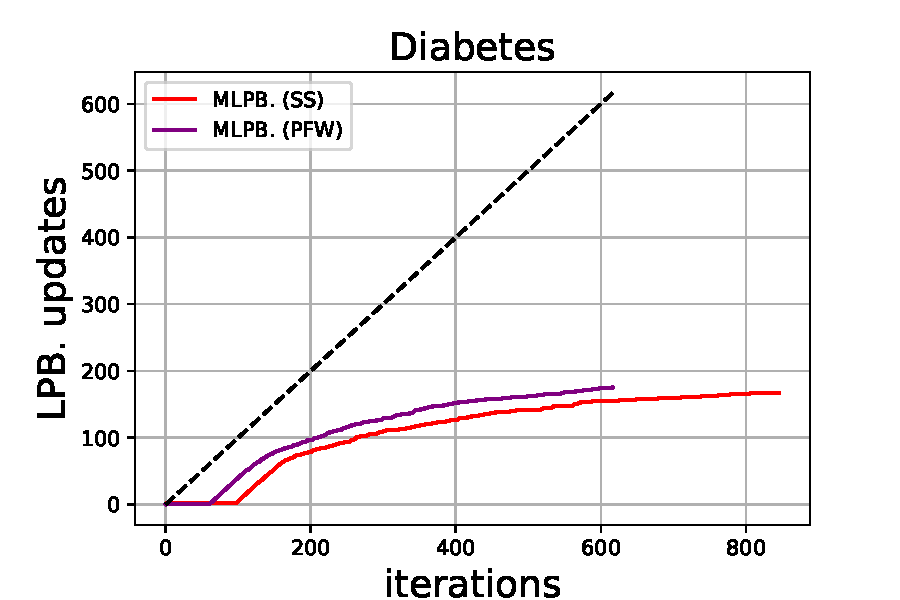
\includegraphics[keepaspectratio, scale=0.30]
            {figure/mlpb_lpb_update_diabetis.pdf}
        \end{minipage}
        \\
        \begin{minipage}[t]{0.31\hsize}
            \centering
            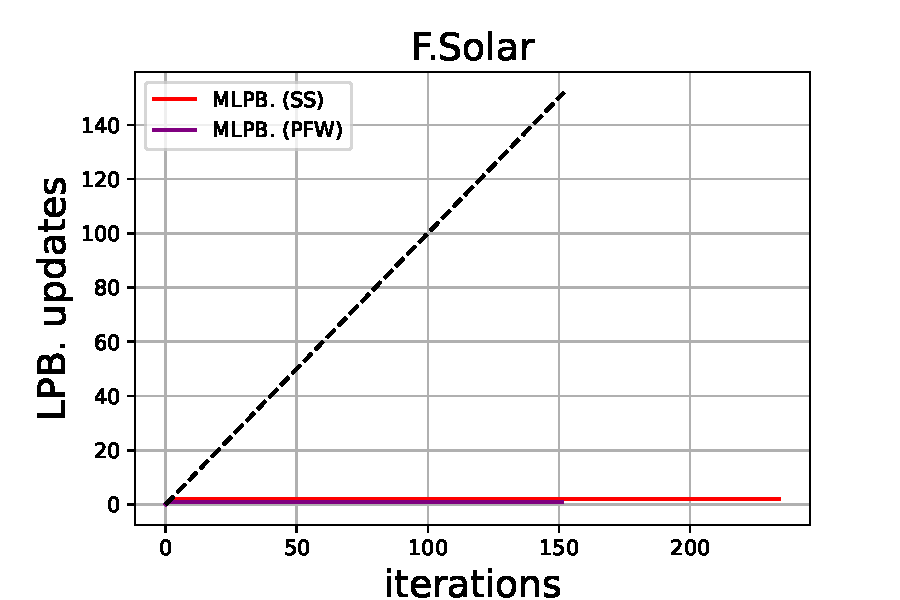
\includegraphics[keepaspectratio, scale=0.30]
            {figure/mlpb_lpb_update_flare_solar.pdf}
        \end{minipage}
        &
        \begin{minipage}[t]{0.31\hsize}
            \centering
            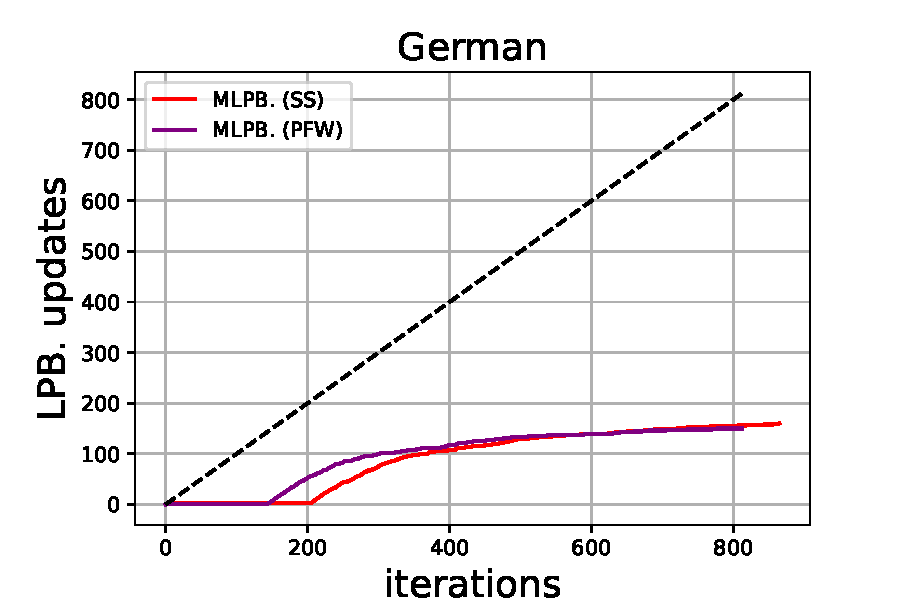
\includegraphics[keepaspectratio, scale=0.30]
            {figure/mlpb_lpb_update_german.pdf}
        \end{minipage}
        &
        \begin{minipage}[t]{0.31\hsize}
            \centering
            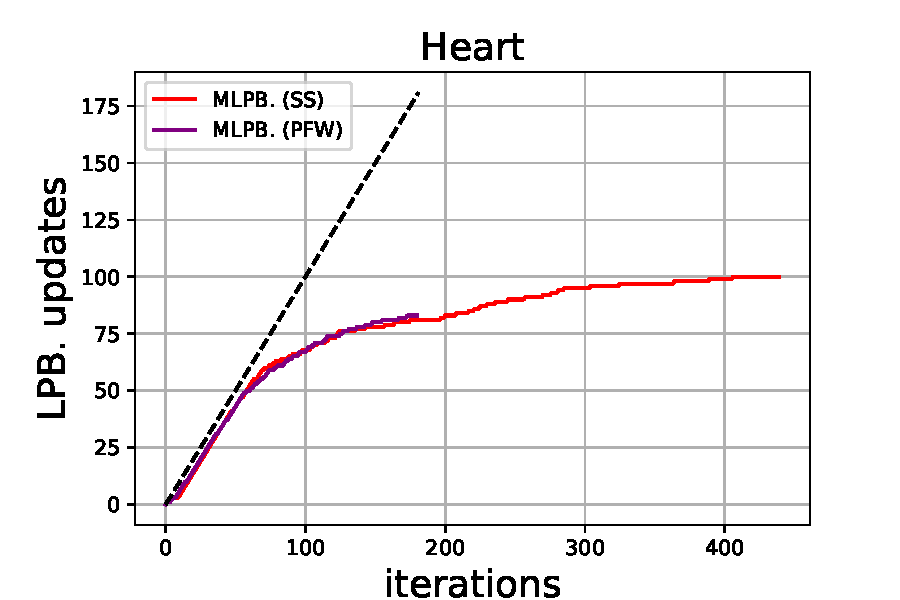
\includegraphics[keepaspectratio, scale=0.30]
            {figure/mlpb_lpb_update_heart.pdf}
        \end{minipage}
        \\
        \begin{minipage}[t]{0.31\hsize}
            \centering
            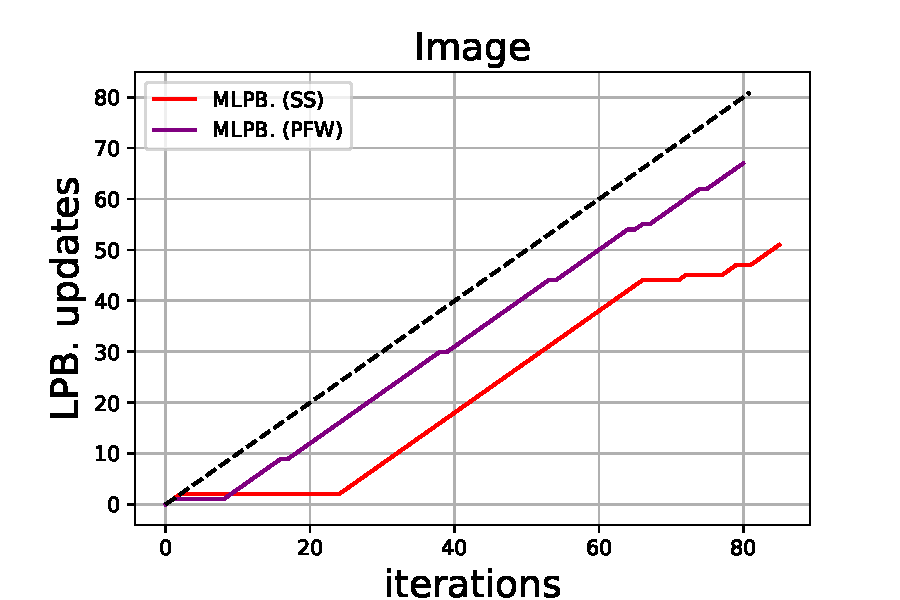
\includegraphics[keepaspectratio, scale=0.30]
            {figure/mlpb_lpb_update_image.pdf}
        \end{minipage}
        &
        \begin{minipage}[t]{0.31\hsize}
            \centering
            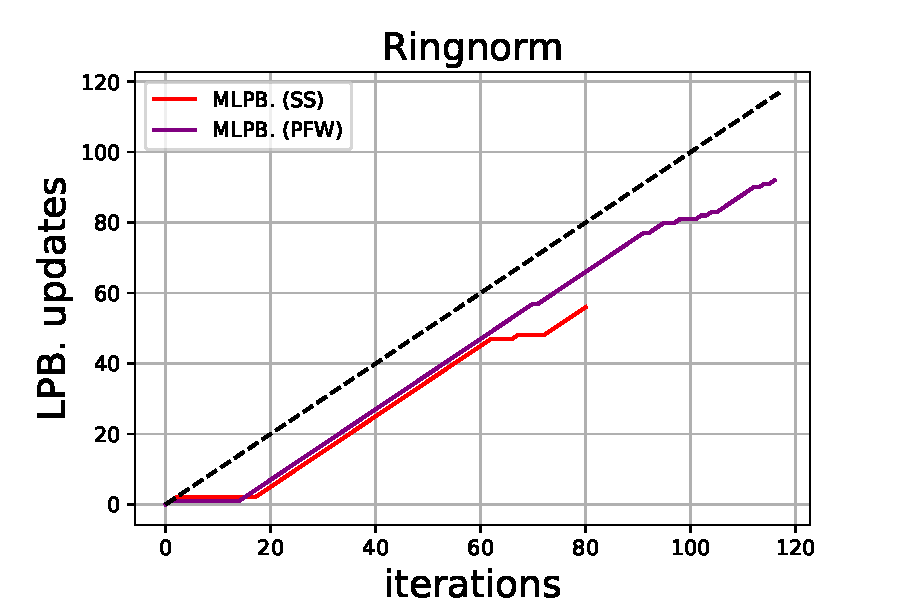
\includegraphics[keepaspectratio, scale=0.30]
            {figure/mlpb_lpb_update_ringnorm.pdf}
        \end{minipage}
        &
        \begin{minipage}[t]{0.31\hsize}
            \centering
            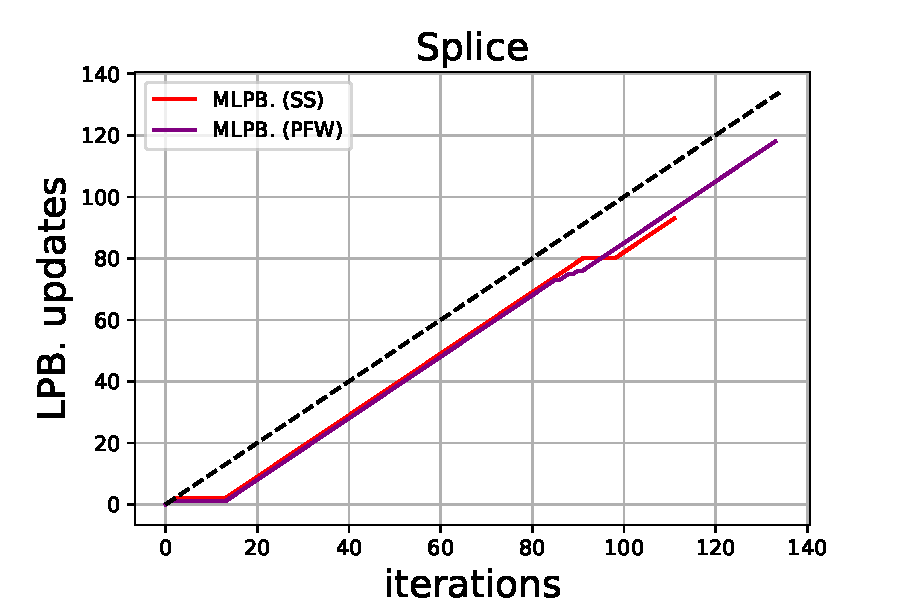
\includegraphics[keepaspectratio, scale=0.30]
            {figure/mlpb_lpb_update_splice.pdf}
        \end{minipage}
        \\
        \begin{minipage}[t]{0.31\hsize}
            \centering
            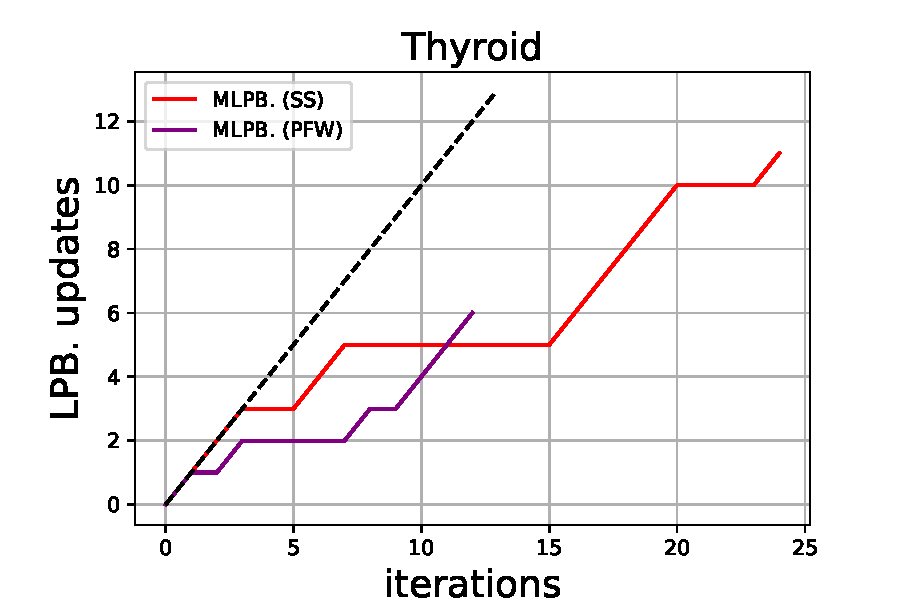
\includegraphics[keepaspectratio, scale=0.30]
            {figure/mlpb_lpb_update_thyroid.pdf}
        \end{minipage}
        &
        \begin{minipage}[t]{0.31\hsize}
            \centering
            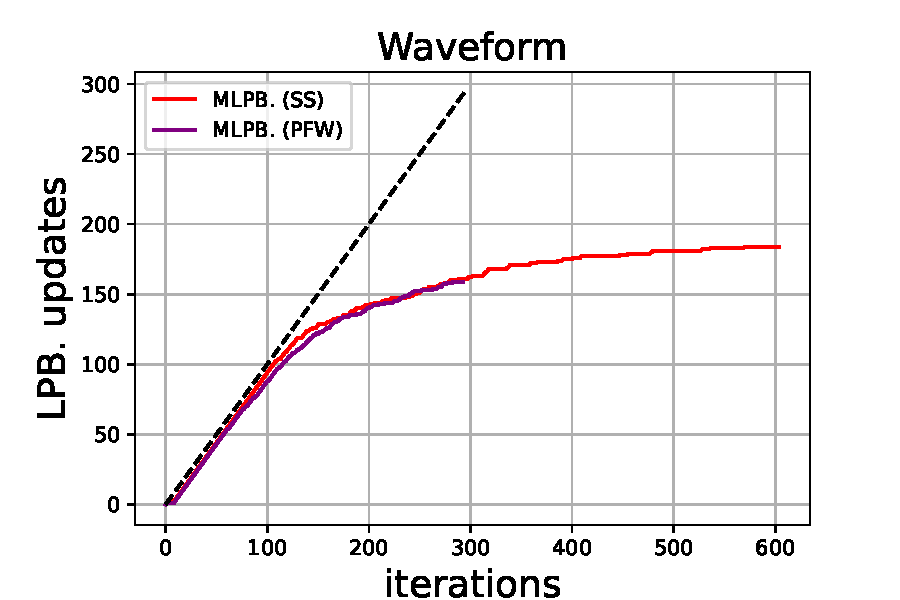
\includegraphics[keepaspectratio, scale=0.30]
            {figure/mlpb_lpb_update_waveform.pdf}
        \end{minipage}
        &
        \begin{minipage}[t]{0.31\hsize}
            \centering
            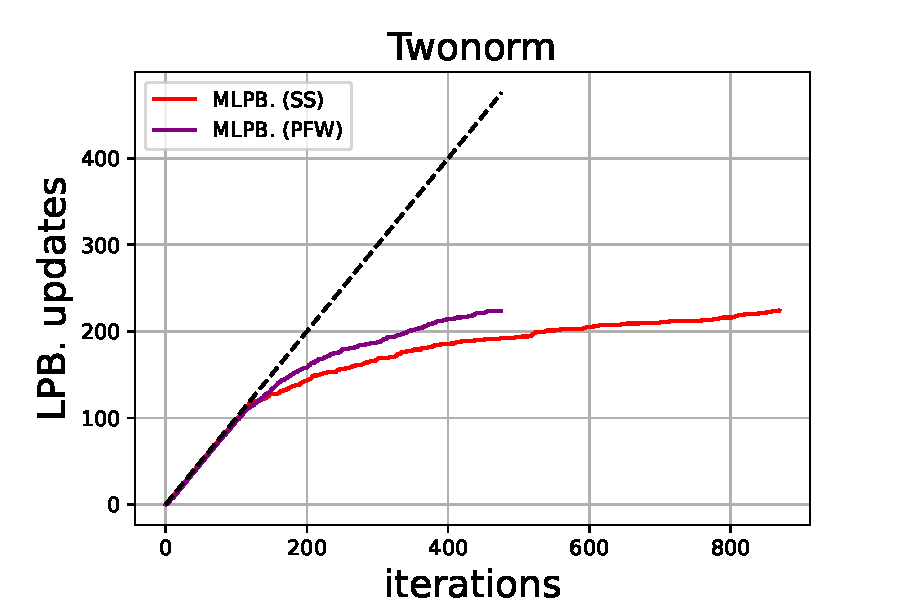
\includegraphics[keepaspectratio, scale=0.30]
            {figure/mlpb_lpb_update_twonorm.pdf}
        \end{minipage}
    \end{tabular}
    \caption{%
        The number of $\secalg$ updates %
        for each benchmark dataset %
        with parameters $\nu = 0.1m$ and $\epsilon = 0.01$. %
        The dotted line indicates the linear function for comparison. %
        Since the shape of the titanic dataset is %
        the same as the F. Solar dataset, %
        we omit it. %
    }
    \label{fig:appendix_lpbcall}
\end{figure}


Finally, we verify the effectiveness of the secondary update $\secalg$, 
shown in algorithm~\ref{alg:lpb_subroutine}. 
For comparison, we measured the soft margin objective and time 
for FW, PFW, MLPB.~(SS), and MLPB.~(PFW). 
FW is the FW algorithm with short-steps, 
and PFW is the Pairwise FW algorithm. 
MLPB.~(SS) and MLPB.~(PFW) are MLPBoosts 
with algorithms~\ref{alg:ss_rule} and~\ref{alg:pairwise_rule}, 
respectively. 
Figure~\ref{fig:appendix_mlpb_compare} shows the results. 
As this figure shows, 
the secondary update $\secalg$ 
improves the objective value significantly. 
\begin{figure}[p]
    \centering
    \begin{tabular}{ccc}
        \begin{minipage}[t]{0.31\hsize}
            \centering
            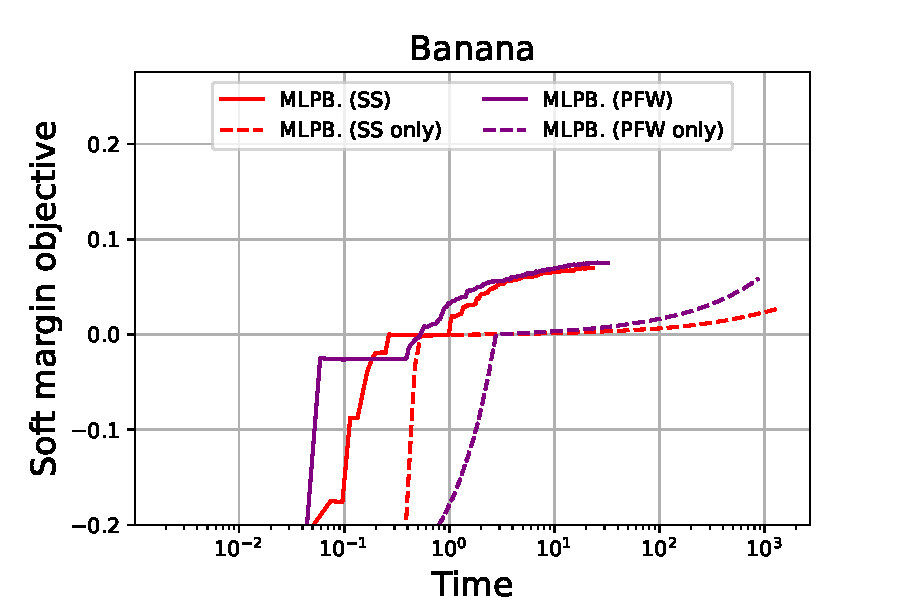
\includegraphics[keepaspectratio, scale=0.30]
            {figure/compare_fw_banana.pdf}
        \end{minipage}
        &
        \begin{minipage}[t]{0.31\hsize}
            \centering
            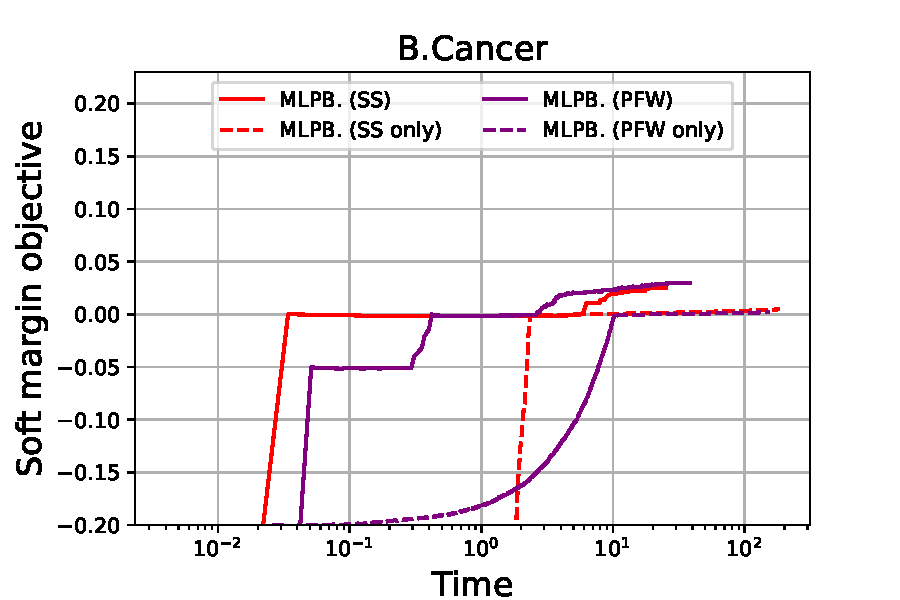
\includegraphics[keepaspectratio, scale=0.30]
            {figure/compare_fw_breast_cancer.pdf}
        \end{minipage}
        &
        \begin{minipage}[t]{0.31\hsize}
            \centering
            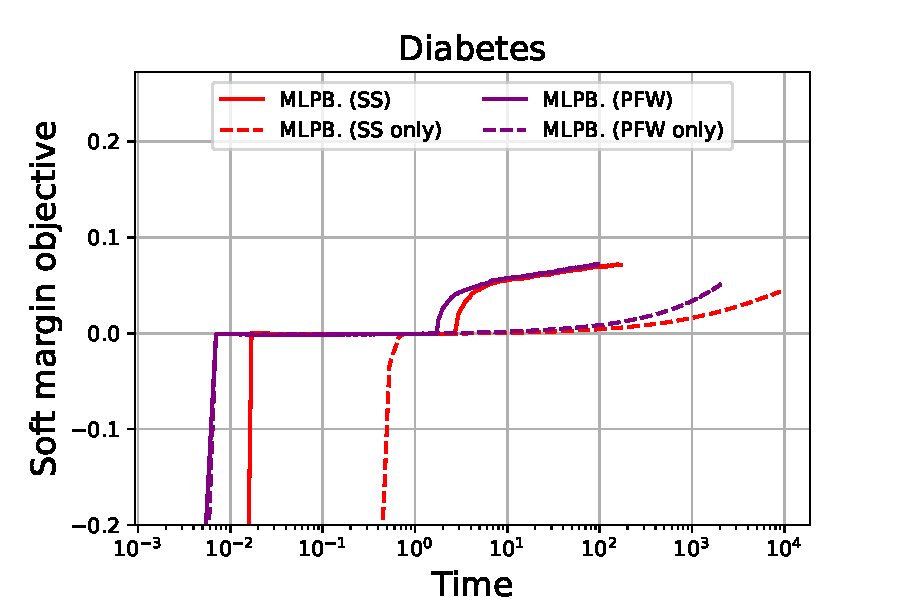
\includegraphics[keepaspectratio, scale=0.30]
            {figure/compare_fw_diabetis.pdf}
        \end{minipage}
        \\
        \begin{minipage}[t]{0.31\hsize}
            \centering
            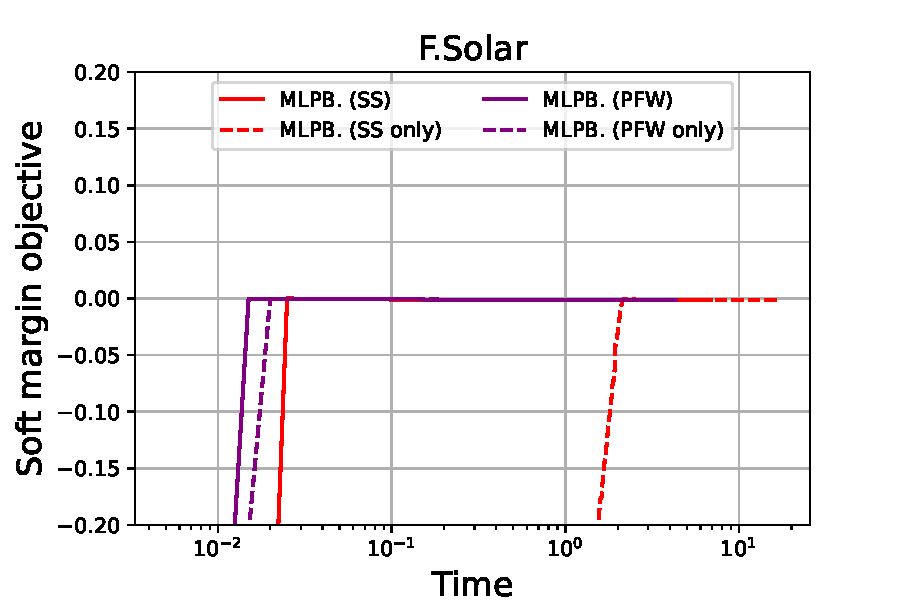
\includegraphics[keepaspectratio, scale=0.30]
            {figure/compare_fw_flare_solar.pdf}
        \end{minipage}
        &
        \begin{minipage}[t]{0.31\hsize}
            \centering
            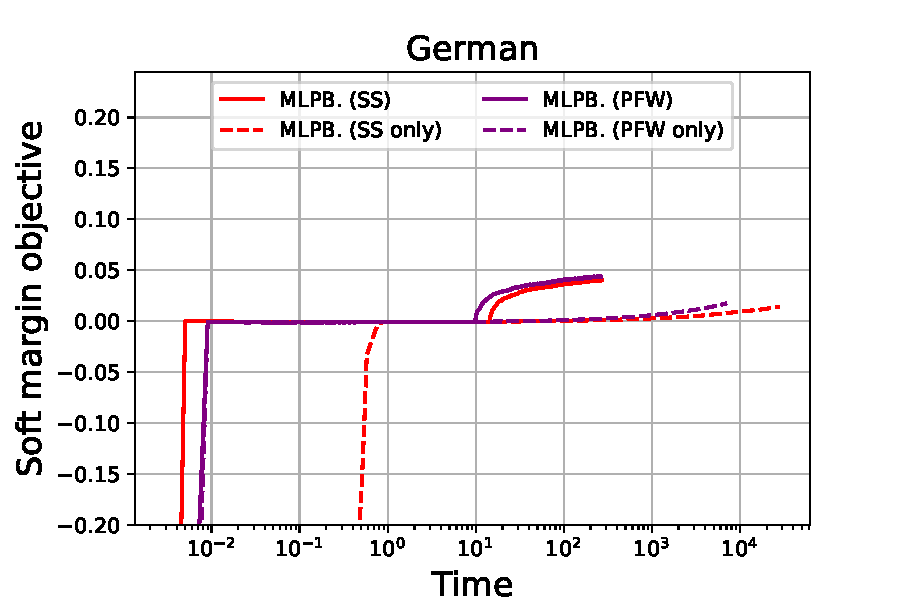
\includegraphics[keepaspectratio, scale=0.30]
            {figure/compare_fw_german.pdf}
        \end{minipage}
        &
        \begin{minipage}[t]{0.31\hsize}
            \centering
            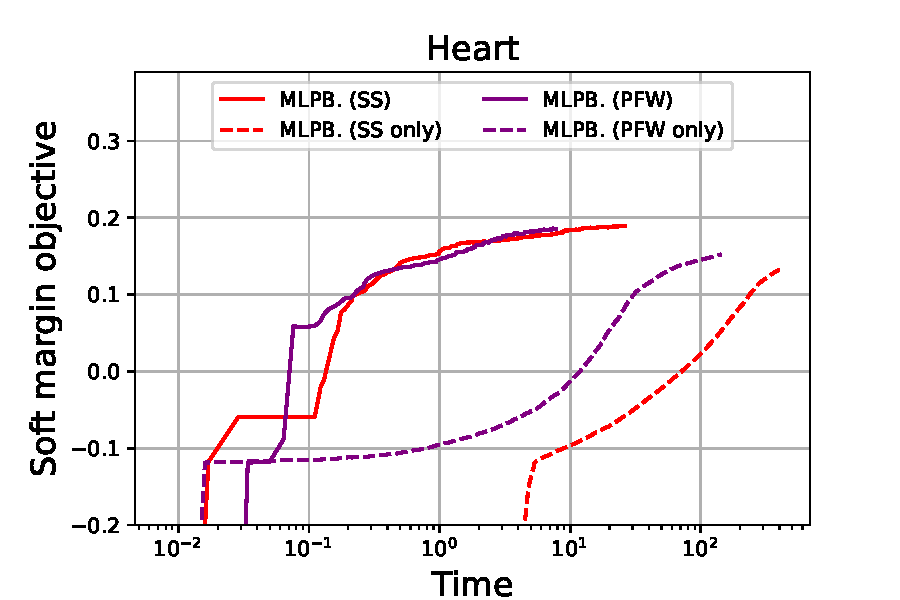
\includegraphics[keepaspectratio, scale=0.30]
            {figure/compare_fw_heart.pdf}
        \end{minipage}
        \\
        \begin{minipage}[t]{0.31\hsize}
            \centering
            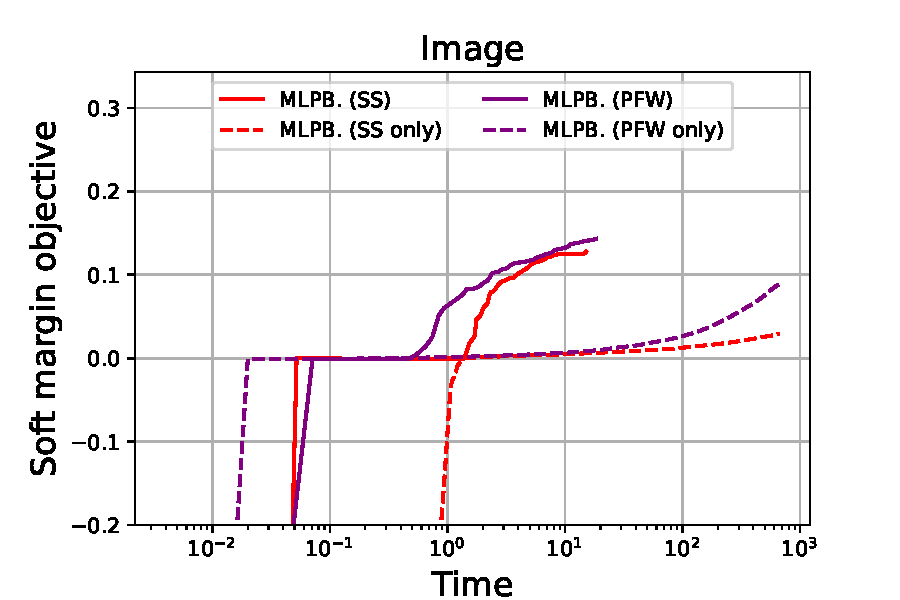
\includegraphics[keepaspectratio, scale=0.30]
            {figure/compare_fw_image.pdf}
        \end{minipage}
        &
        \begin{minipage}[t]{0.31\hsize}
            \centering
            \includegraphics[keepaspectratio, scale=0.30]
            {figure/compare_fw_ringnorm.pdf}
        \end{minipage}
        &
        \begin{minipage}[t]{0.31\hsize}
            \centering
            \includegraphics[keepaspectratio, scale=0.30]
            {figure/compare_fw_splice.pdf}
        \end{minipage}
        \\
        \begin{minipage}[t]{0.31\hsize}
            \centering
            \includegraphics[keepaspectratio, scale=0.30]
            {figure/compare_fw_thyroid.pdf}
        \end{minipage}
        &
        \begin{minipage}[t]{0.31\hsize}
            \centering
            \includegraphics[keepaspectratio, scale=0.30]
            {figure/compare_fw_waveform.pdf}
        \end{minipage}
        &
        \begin{minipage}[t]{0.31\hsize}
            \centering
            \includegraphics[keepaspectratio, scale=0.30]
            {figure/compare_fw_twonorm.pdf}
        \end{minipage}
    \end{tabular}
    \caption{%
        Comparison of the FW algorithms and MLPBoosts. %
        As this figure shows, the secondary update $\secalg$ yields %
        huge progress. %
    }
    \label{fig:appendix_mlpb_compare}
\end{figure}

\end{document}

